\documentclass[a4paper,12pt]{article}
\usepackage{geometry}
\usepackage{amsmath,amsfonts,amssymb}
\usepackage{graphicx}
\usepackage{subcaption}
\usepackage{caption}
\usepackage{booktabs}
\usepackage{hyperref}
\usepackage{enumitem}
\usepackage{xcolor}
\usepackage{titling}
\usepackage{fancyhdr}
\usepackage{parskip}
\usepackage{float}

% Custom colors
\definecolor{titleblue}{RGB}{0,102,204}
\definecolor{headingblue}{RGB}{0,51,102}

% Page layout
\geometry{top=2.5cm,bottom=2.5cm,left=2.5cm,right=2.5cm}
\setlength{\parindent}{0pt}
\setlength{\parskip}{1em}

% Header and footer
\pagestyle{fancy}
\fancyhf{}
\fancyhead[L]{\textbf{INS3155 -- Computer Vision Midterm Report}}
\fancyhead[R]{\thetitle}
\fancyfoot[C]{\thepage}

% Title customization
\pretitle{\centering\LARGE\bfseries}
\posttitle{\vspace{0.5cm}}
\preauthor{\centering}
\postauthor{}
\predate{\centering}
\postdate{}

\begin{document}

\title{\textcolor{titleblue}{Midterm Project Report}}

\author{\parbox{0.6\linewidth}{\centering
Name: Pham Ho Bao\\
Student ID: 23070455\\
Email: 23070455@student.hcmus.edu.vn}}

\date{\today}

\maketitle

% ============================================================
% ABSTRACT
% ============================================================
\begin{abstract}
This report presents the systematic implementation and quantitative evaluation of three foundational computer vision pipelines: (1) spatial-domain image filtering and restoration, (2) 3D reconstruction from stereo images via disparity mapping, and (3) multi-view image stitching for panorama generation. For image filtering, five spatial filters---Mean, Gaussian, Median, Laplacian, and Bilateral---were benchmarked against Gaussian and Salt \& Pepper noise using PSNR and SSIM metrics. The Median filter achieved 33.36~dB PSNR against impulse noise, while the Gaussian filter reached 30.16~dB against additive noise. In stereo reconstruction, Semi-Global Block Matching (SGBM) recovered 103,441 valid 3D points with superior coherence over standard Block Matching. For panorama stitching, SIFT produced 2.18$\times$ more feature matches than ORB, while ORB executed 2.0$\times$ faster, establishing application-specific trade-offs between accuracy and real-time performance.
\end{abstract}

% ============================================================
% 1. INTRODUCTION
% ============================================================
\section{Introduction}

Computer vision fundamentally seeks to algorithmically comprehend, restore, and extract spatial and semantic information from digital imagery. This midterm project systematically explores three foundational pillars of the discipline: 2D image restoration (Part~A), 3D structural reconstruction (Part~B), and multi-view geometric alignment (Part~C).

\textbf{Motivation:}
In real-world visual systems, raw image data is inherently imperfect---corrupted by sensor noise, confined to two-dimensional planar projections, and restricted by the limited field of view of a single camera lens. This laboratory addresses these ubiquitous challenges sequentially. First, we investigate how to neutralize signal degradation while preserving high-frequency image borders through spatial domain filtering. Next, we upgrade from 2D pixel matrices to 3D point clouds by exploiting binocular parallax, unlocking depth perception crucial for robotics and autonomous navigation. Finally, we bypass hardware sensor limitations by algorithmically stitching discrete snapshots into cohesive panoramic environments using robust feature tracking.

By mathematically verifying these classical computer vision theories against programmatic implementations, this report establishes a concrete understanding of local gradient operations, epipolar geometry, and scale-invariant robust estimators.

% ============================================================
% 2. PART A: IMAGE FILTERING AND RESTORATION
% ============================================================
\section{Part A: Image Filtering and Restoration}

\subsection{Methods and Mathematical Foundations}

Image degradation was rigorously simulated by injecting two distinct stochastic noise profiles:

\begin{itemize}
    \item \textbf{Gaussian Noise (Additive):} Statistical noise modeling camera sensor/thermal noise, defined by $I_{noisy} = I_{orig} + \mathcal{N}(0, \sigma^2)$. It corrupts all pixels systemically.
    \item \textbf{Salt \& Pepper Noise (Impulse):} Sparse noise modeling transmission errors or dead sensor pixels, where a subset of pixels is forced to absolute extremes (e.g., probability $P/2$ for 0 and $P/2$ for 255).
\end{itemize}

To restore the degraded structural information, five spatial domain filters were evaluated:

\begin{itemize}
    \item \textbf{Mean Filter}: Simple block averaging---each pixel is replaced by the arithmetic mean of its local $k \times k$ neighborhood:
    \begin{equation}
        \hat{I}(x,y) = \frac{1}{k^2} \sum_{i=-a}^{a} \sum_{j=-a}^{a} I(x+i, y+j)
    \end{equation}
    where $a = \lfloor k/2 \rfloor$. Operates in $O(k^2)$, or $O(1)$ using integral images.

    \item \textbf{Gaussian Filter}: Convolution with a 2D Gaussian distribution $G(x,y) = \frac{1}{2\pi\sigma^2}e^{-\frac{x^2+y^2}{2\sigma^2}}$. Unlike the Mean filter, the Gaussian kernel is mathematically \textit{separable}, allowing the $O(k^2)$ 2D convolution to be optimized into two 1D passes with $O(2k)$ computational complexity.

    \item \textbf{Median Filter}: Non-linear rank-order filter that replaces each pixel with the median value of its neighborhood $\hat{I}(x,y) = \text{median}\{I(x+i, y+j) \mid i,j \in [-a, a]\}$. Because statistical rank ordering naturally excludes extreme minimums and maximums, it is theoretically optimal for eliminating impulse noise outliers.

    \item \textbf{Laplacian Filter}: A 2nd-order isotropic derivative operator $\nabla^2 I = \frac{\partial^2 I}{\partial x^2} + \frac{\partial^2 I}{\partial y^2}$. Because it emphasizes high-frequency spatial gradients, it highlights edges but inherently \textit{amplifies} existing noise---it is benchmarked here to demonstrate its failure mode as a denoiser.

    \item \textbf{Bilateral Filter}~\cite{tomasi1998bilateral}: An edge-preserving filter that combines a spatial Gaussian kernel ($G_{\sigma_s}$) with an intensity-range Gaussian kernel ($G_{\sigma_r}$). The restored pixel at position $\mathbf{p}$ is:
    \begin{equation}
        BF[I]_\mathbf{p} = \frac{1}{W_\mathbf{p}} \sum_{\mathbf{q} \in S} G_{\sigma_s}(\|\mathbf{p} - \mathbf{q}\|) \, G_{\sigma_r}(|I_\mathbf{p} - I_\mathbf{q}|) \, I_\mathbf{q}
    \end{equation}
    where $W_\mathbf{p}$ is the normalization term. It weights adjacent pixels heavily \textit{only if} they have similar intensity context, meaning the weight drops to near-zero right across geometric boundaries, preserving sharp edges while smoothing homogenous regions.
\end{itemize}

\subsubsection{Architectural Rationale: Why, Where, and How}

To fully understand the pipeline, it is crucial to explicitly establish \textbf{why} certain filters were chosen, \textbf{where} they are best deployed, and \textbf{how} their mathematical mechanics interact with the noise and each other:

\begin{itemize}
    \item \textbf{The Linear Averages (Mean \& Gaussian):}
    \begin{itemize}
        \item \textit{Why \& Where:} Deployed specifically to combat Gaussian (additive) noise. Because Gaussian noise shifts pixel values across a normal distribution with a mean of zero, calculating the local spatial average naturally cancels out the noise perturbations. They are used in baseline hardware sensors where computational speed is prioritized.
        \item \textit{How they interact:} The Mean filter blindly treats all neighborhood pixels equally, causing severe structural blurring. The Gaussian filter interacts more intelligently by weighting central pixels higher, yielding a vastly better SSIM (structural perception) and avoiding the ``box-blur'' artifact, despite performing the same fundamental noise-canceling task.
    \end{itemize}

    \item \textbf{The Non-Linear Approach (Median):}
    \begin{itemize}
        \item \textit{Why \& Where:} Chosen exclusively as a targeted countermeasure to Salt \& Pepper (impulse) noise. It is deployed in scenarios plagued by transmission failures, dead sensor pixels, or bit-flip errors.
        \item \textit{How it interacts:} Impulse noise injects mathematical extreme outliers (0 or 255). If fed into a linear spatial filter, these extreme values are absorbed and smeared uniformly into the local average, permanently destroying the surrounding topology. The Median filter bypasses this completely by dropping the extremities from its sorted rank, directly pushing the algebraic error (MSE) down and rocketing the PSNR back up to $>31$~dB without the side-effect of edge-blur.
    \end{itemize}

    \item \textbf{The Edge-Preserving Mechanism (Bilateral):}
    \begin{itemize}
        \item \textit{Why \& Where:} Deployed as the optimal offline denoiser for aesthetically sensitive or edge-critical images suffering from Gaussian noise (e.g., consumer photography, medical MRI/CT scans).
        \item \textit{How it interacts:} It intertwines spatial distance with color distance. When the filter convolution window overlaps an object boundary, the sharp color discrepancy forces the internal weight to drop to zero, acting like a dynamic barrier. This ensures Gaussian smoothing happens \textit{only} inside flat, homogenous regions, leaving geometric boundaries perfectly intact.
    \end{itemize}
\end{itemize}

\subsubsection{Evaluation Metrics}

To quantitatively evaluate the effectiveness of noise removal and algorithm interaction, we compute two complementary metrics:

\textbf{Peak Signal-to-Noise Ratio (PSNR)}---measures pixel-level reconstruction accuracy:
\begin{equation}
    \text{MSE} = \frac{1}{M \cdot N} \sum_{i=0}^{M-1} \sum_{j=0}^{N-1} [I_{original}(i,j) - I_{restored}(i,j)]^2
\end{equation}
\begin{equation}
    \text{PSNR} = 10 \cdot \log_{10} \left( \frac{\text{MAX}_I^2}{\text{MSE}} \right)
\end{equation}
where $\text{MAX}_I$ is the maximum possible pixel value (e.g., 255 for 8-bit images), and MSE is the Mean Squared Error between the original and restored image.

\textbf{Structural Similarity Index (SSIM)}~\cite{wang2004image}---mathematically models human visual perception. Rather than treating all pixel errors equally, SSIM evaluates structural distortion, luminance shifts, and contrast changes:
\begin{equation}
    \text{SSIM}(x,y) = \frac{(2\mu_x\mu_y + c_1)(2\sigma_{xy} + c_2)}{(\mu_x^2 + \mu_y^2 + c_1)(\sigma_x^2 + \sigma_y^2 + c_2)}
\end{equation}
where $\mu_x, \mu_y$ are local block means (luminance), $\sigma_x, \sigma_y$ are local standard deviations (contrast), $\sigma_{xy}$ is the cross-covariance (structure), and $c_1, c_2$ are stabilizing constants preventing division by zero. SSIM ranges from 0 (no structural correlation) to 1 (identical).

% -------------------------------------------------------
\subsection{Implementation \& Qualitative Results}

We implemented the filtering pipeline using Python and OpenCV~\cite{bradski2000opencv}. To visually evaluate the mathematical effects of the filters, we present qualitative results using a kernel size of $k=5$.

\subsubsection{Original and Noisy Context Observation}

The Gaussian noise injection ($\sigma^2$ variance) creates a uniform, ``grainy'' overlay that obscures fine textures but retains the global structure. In contrast, the Salt \& Pepper impulse noise obliterates structural data completely at randomly chosen pixels, leaving stark black and white topological ``holes'' across the image.

\begin{figure}[H]
    \centering
    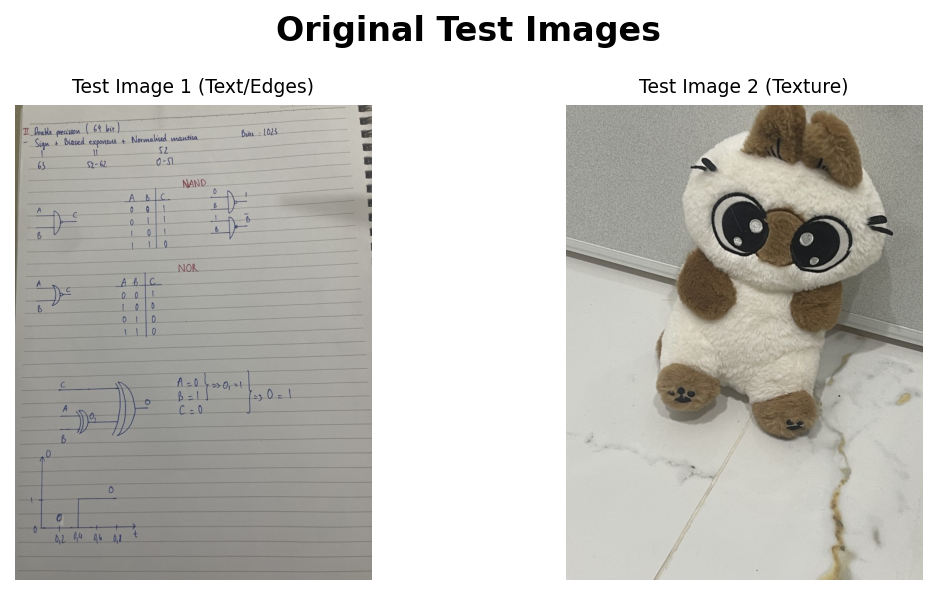
\includegraphics[width=0.9\textwidth]{results/part_a/original_images.png}
    \caption{Original test images before noise injection.}
    \label{fig:original_images}
\end{figure}

\begin{figure}[H]
    \centering
    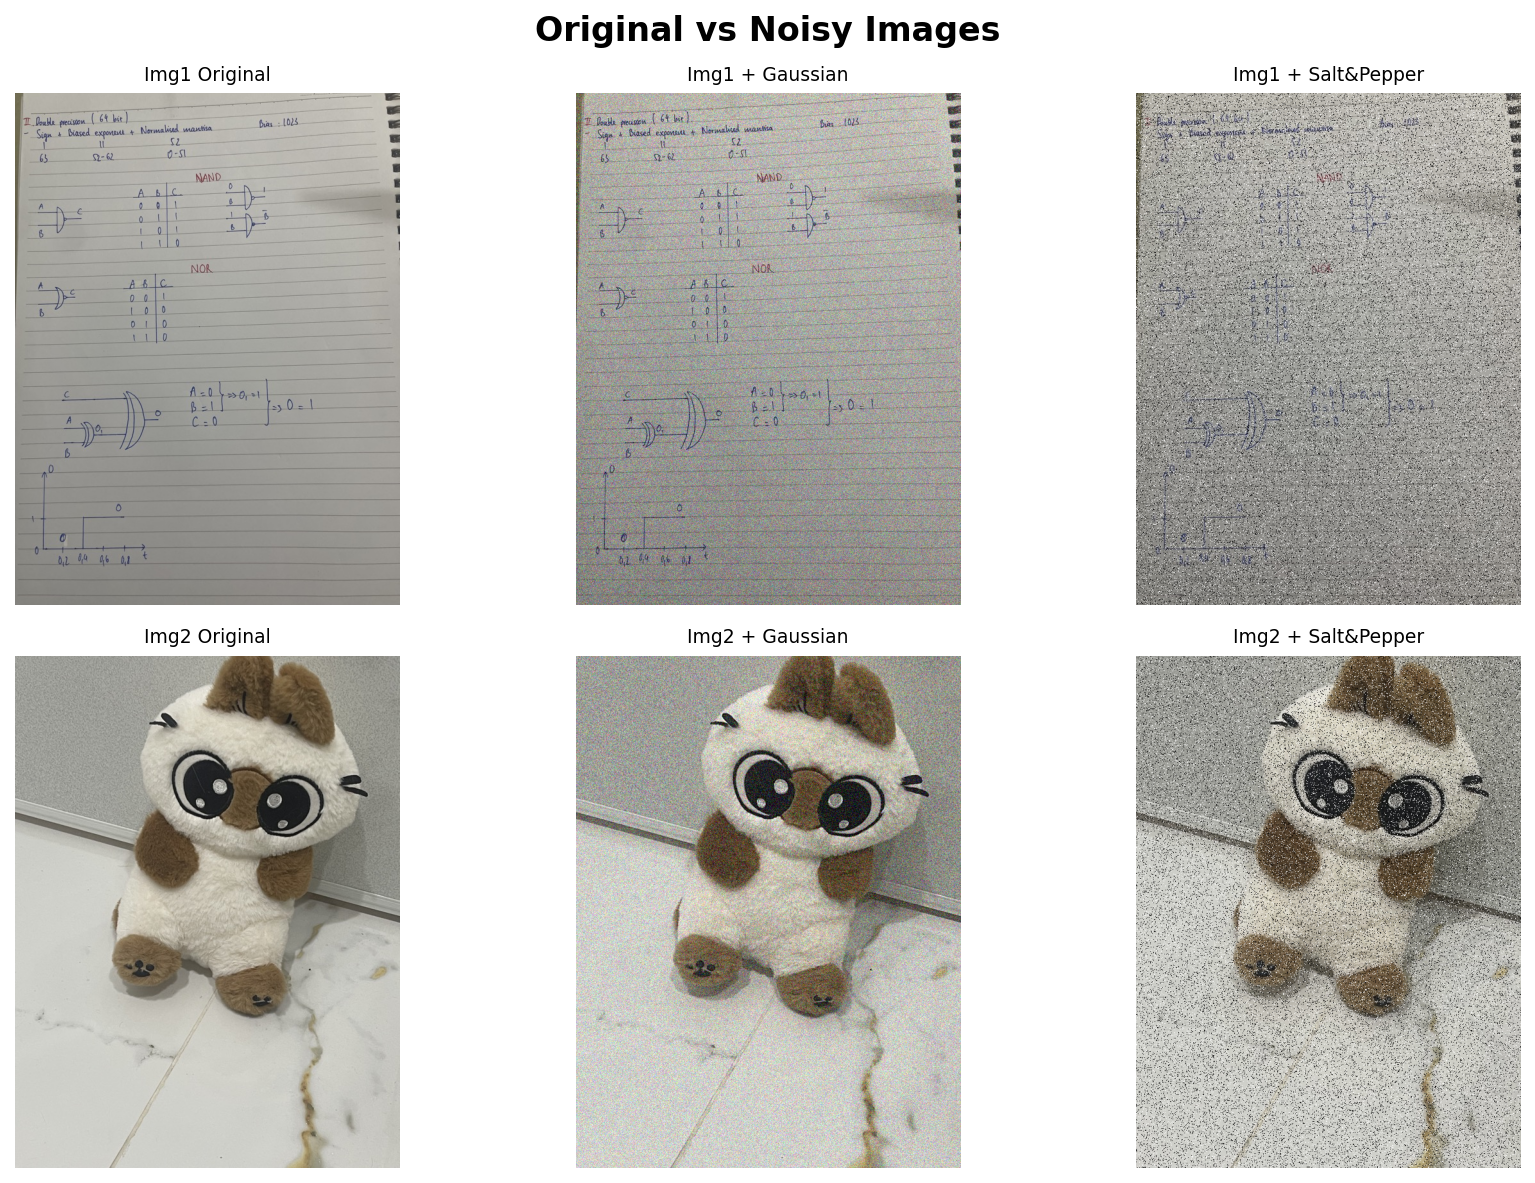
\includegraphics[width=0.9\textwidth]{results/part_a/noisy_images.png}
    \caption{Images corrupted with Gaussian noise (left) and Salt \& Pepper noise (right).}
    \label{fig:noisy_images}
\end{figure}

\subsubsection{Qualitative Restoration Analysis: Gaussian Noise}

When deploying the filters against Gaussian noise, distinct visual behaviors emerge:
\begin{enumerate}
    \item The \textbf{Mean filter} forcefully removes the grain but introduces severe ``box-blurring'', irreparably damaging sharp edges.
    \item The \textbf{Gaussian filter} provides a much smoother, natural blur due to its central weighting, but still fails to respect object boundaries.
    \item The \textbf{Bilateral filter} proves qualitatively superior: the homogenous backgrounds are scrubbed clean of noise, while high-contrast boundary lines (edges) remain distinctly sharp, confirming its edge-preserving geometry.
    \item The \textbf{Laplacian filter} completely fails as a denoiser, resulting in a dark, high-contrast scattered map. Because Laplacian relies on 2nd-order derivatives, it misinterprets the random noise fluctuations as physical edges and visually amplifies them.
\end{enumerate}

\begin{figure}[H]
    \centering
    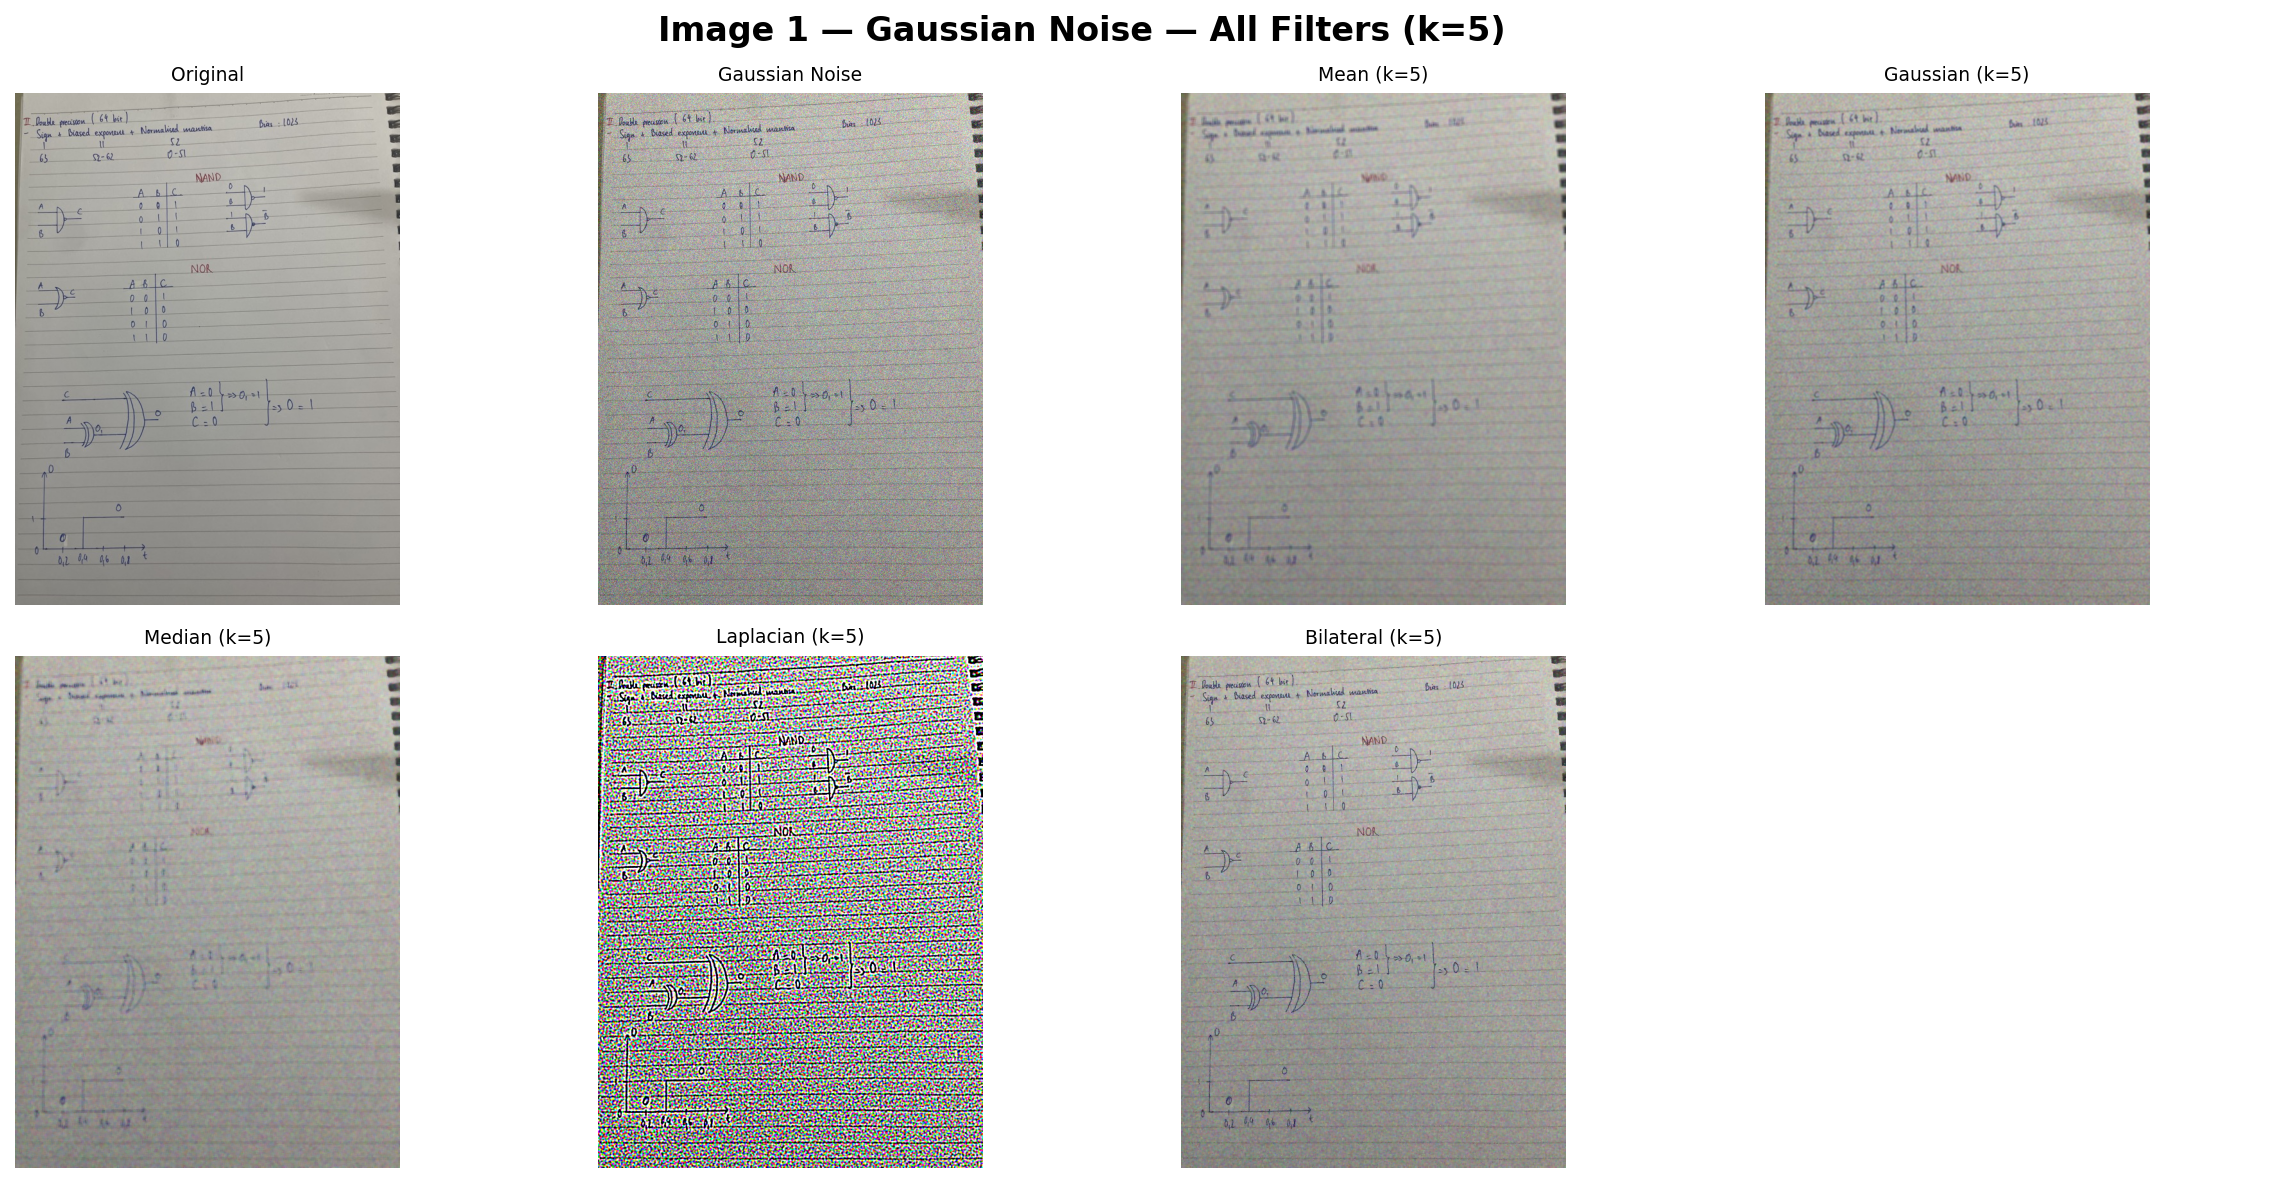
\includegraphics[width=0.95\textwidth]{results/part_a/filters_gaussian_noise_k5.png}
    \caption{Filter restoration results on Gaussian noise ($k=5$).}
    \label{fig:filters_gaussian}
\end{figure}

\subsubsection{Qualitative Restoration Analysis: Salt \& Pepper Noise}

When faced with extreme mathematical impulses (0 or 255), linear filters collapse:
\begin{enumerate}
    \item The \textbf{Mean and Gaussian filters} absorb the extreme outlier pixels into their local averages. Visually, this creates ``smears''---the white and black dots bleed into the surrounding healthy pixels, creating a permanent grey, mottled artifacting that ruins the image structure.
    \item The \textbf{Bilateral filter} attempts to block these extreme outliers from blending by treating them as edges (due to the stark color difference), but this paradoxically traps the noise in place, failing to remove it.
    \item The \textbf{Median filter} completely eradicates the issue. Because the filter ranks pixels and strictly selects the median sequence, the extreme 0 and 255 values are permanently discarded. The visual result is a pristine restoration that rivals the original image, with virtually zero blur introduced.
\end{enumerate}

\begin{figure}[H]
    \centering
    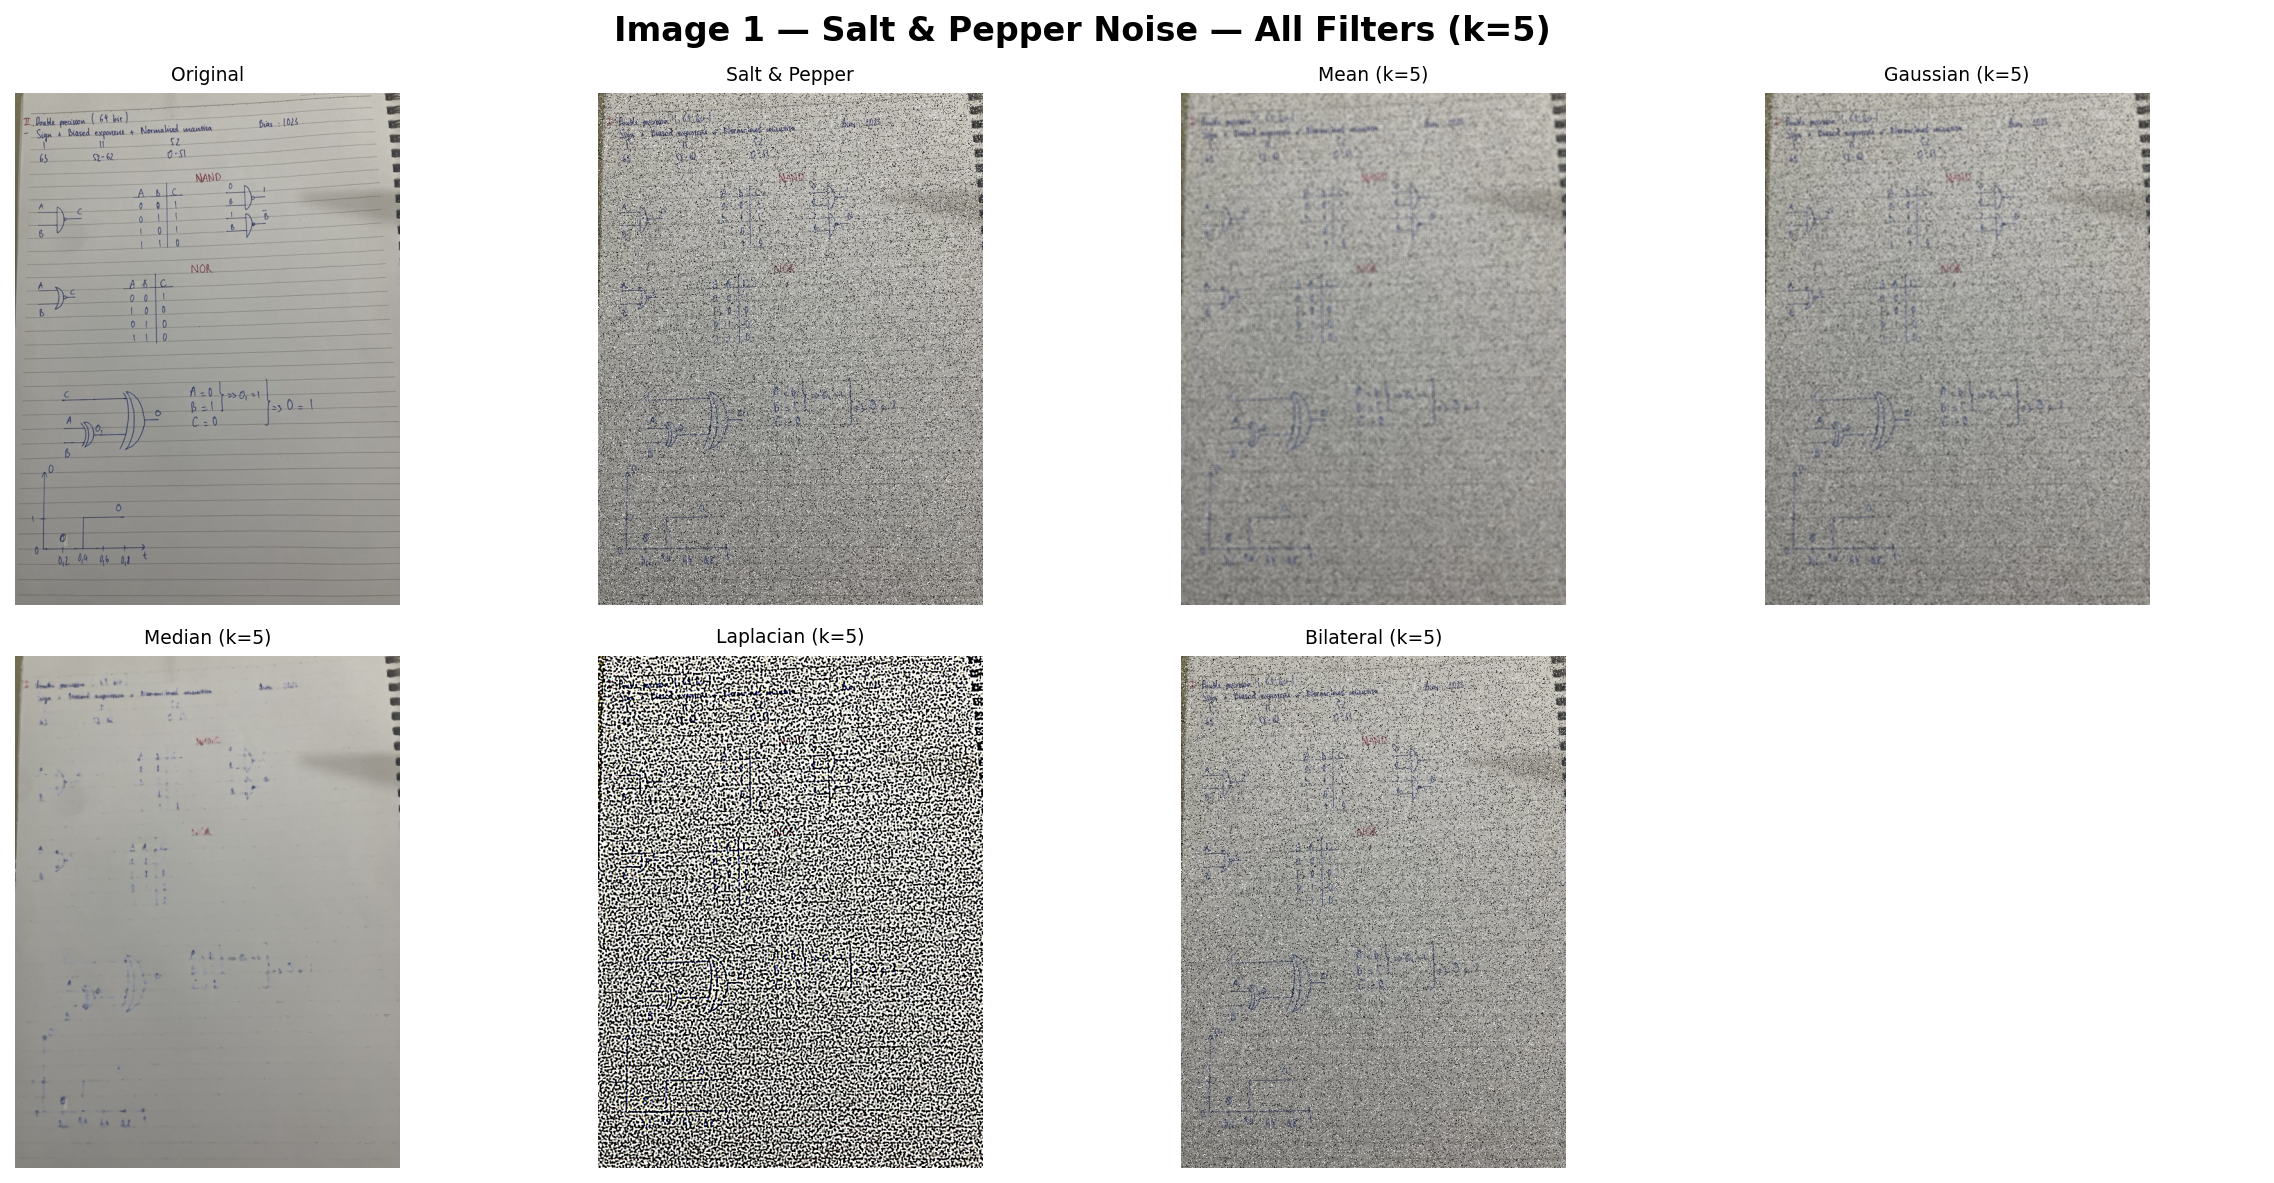
\includegraphics[width=0.95\textwidth]{results/part_a/filters_sp_noise_k5.png}
    \caption{Filter restoration results on Salt \& Pepper noise ($k=5$).}
    \label{fig:filters_sp}
\end{figure}

\subsubsection{Advanced Observation: Edge Preservation \& Kernel Size Impact}

To truly appreciate the architectural difference between a blind linear blur and an edge-preserving filter, observing a zoomed-in topological boundary is critical. Below, the \textbf{edge preservation comparison} explicitly shows how the Bilateral filter erects an mathematical barrier at color thresholds to keep edges sharp, while standard Gaussian convolution bleeds over the boundary.

\begin{figure}[H]
    \centering
    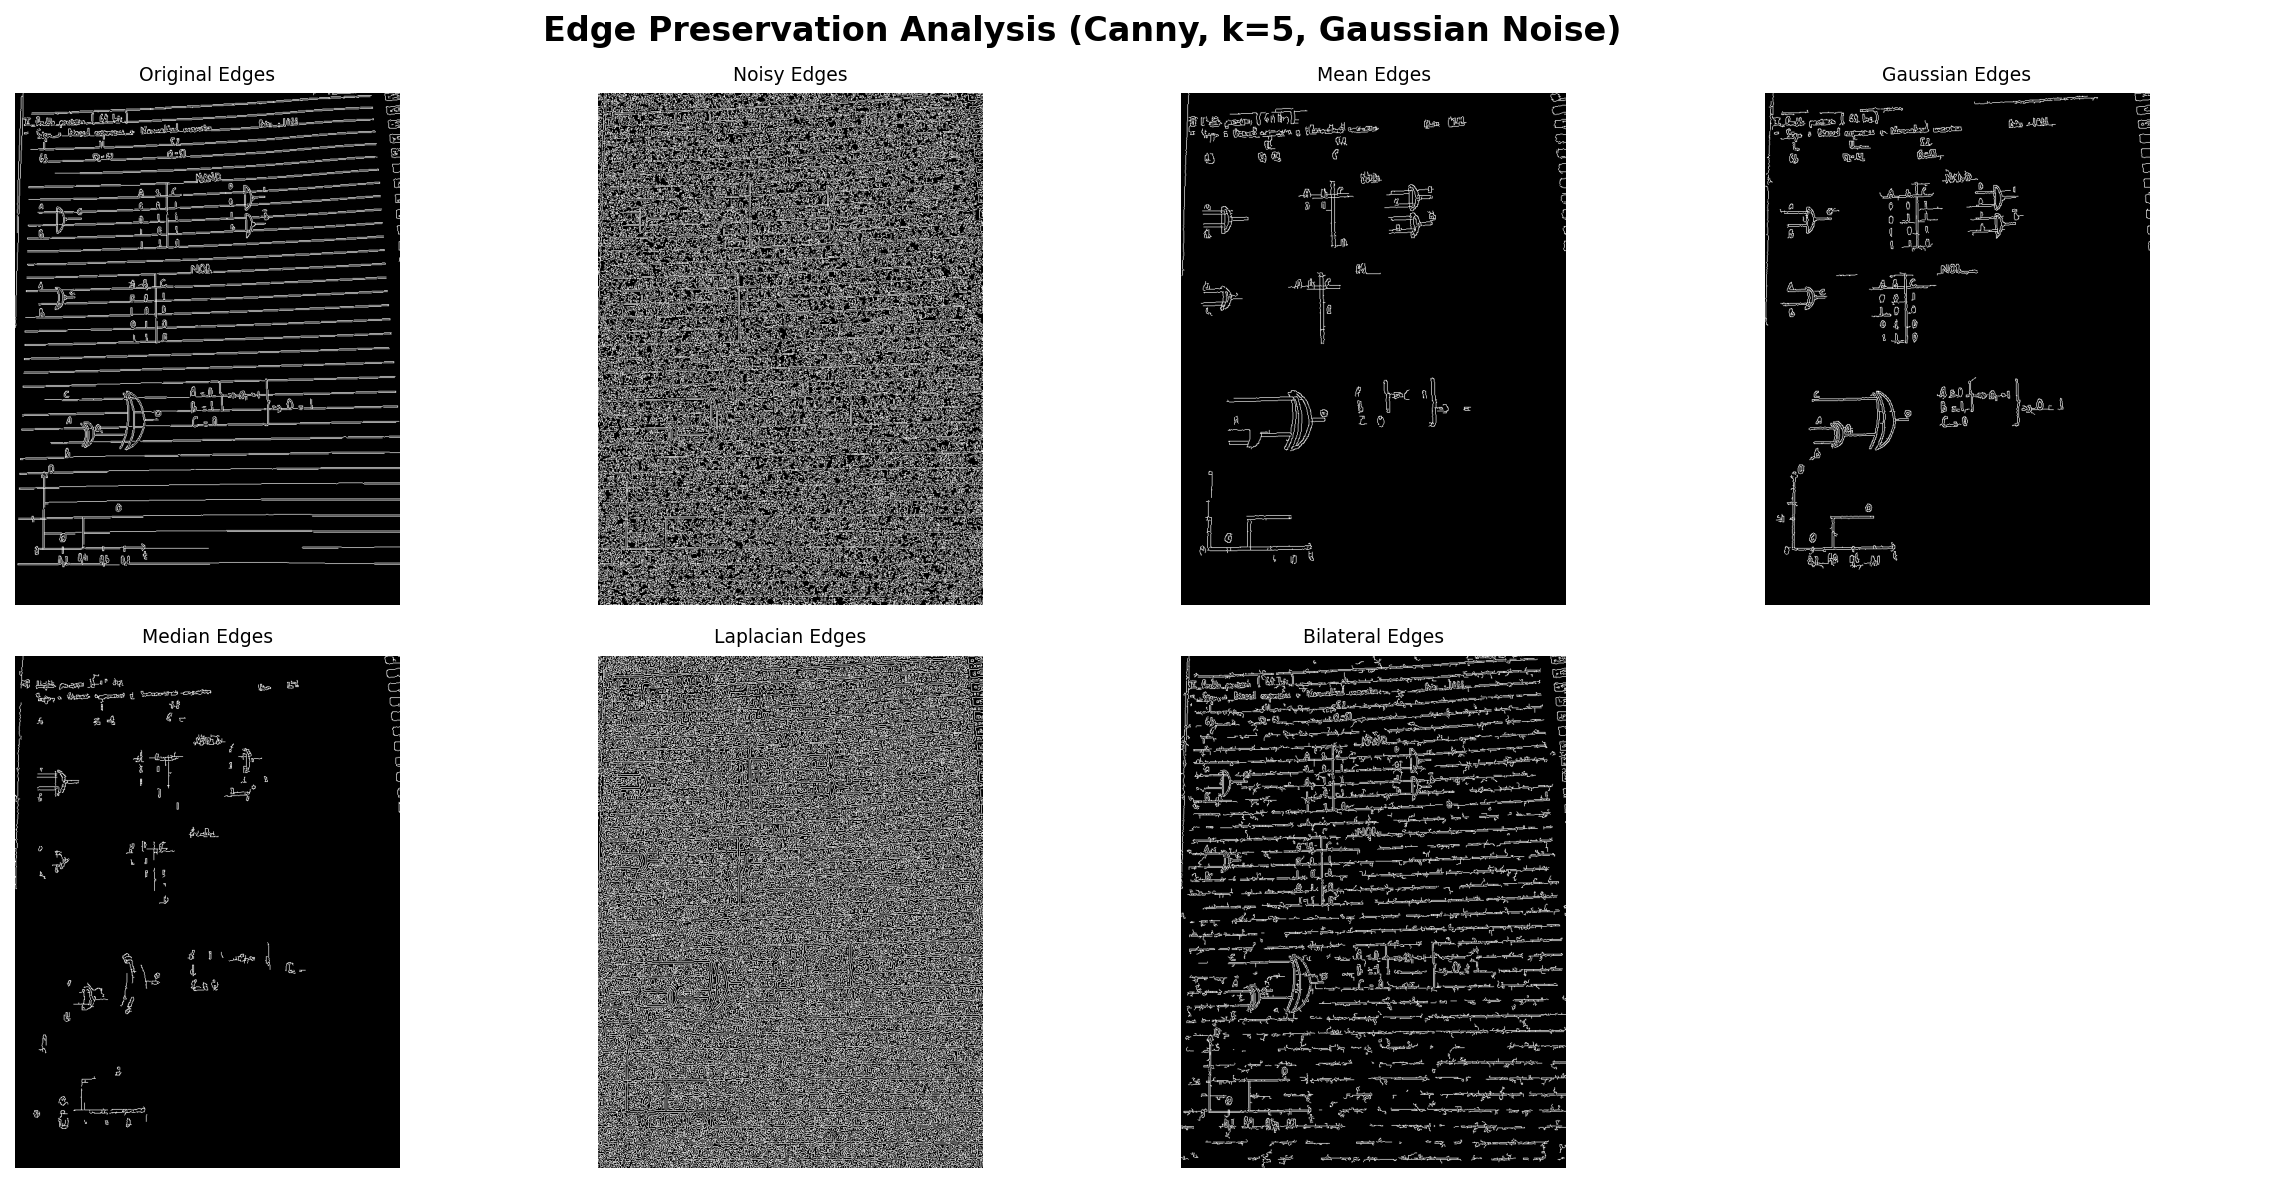
\includegraphics[width=0.85\textwidth]{results/part_a/edge_preservation.png}
    \caption{Edge preservation comparison: Bilateral filter vs.\ Gaussian filter on a zoomed boundary region.}
    \label{fig:edge_preservation}
\end{figure}

Furthermore, the size of the convolution window (Kernel size $k$) forces a significant mathematical trade-off. As $k$ increases, Gaussian filters smooth out vast areas of noise effectively (higher smoothing power), but median filters pull data from too far away, structurally warping small details like text and sharp corners.

\begin{figure}[H]
    \centering
    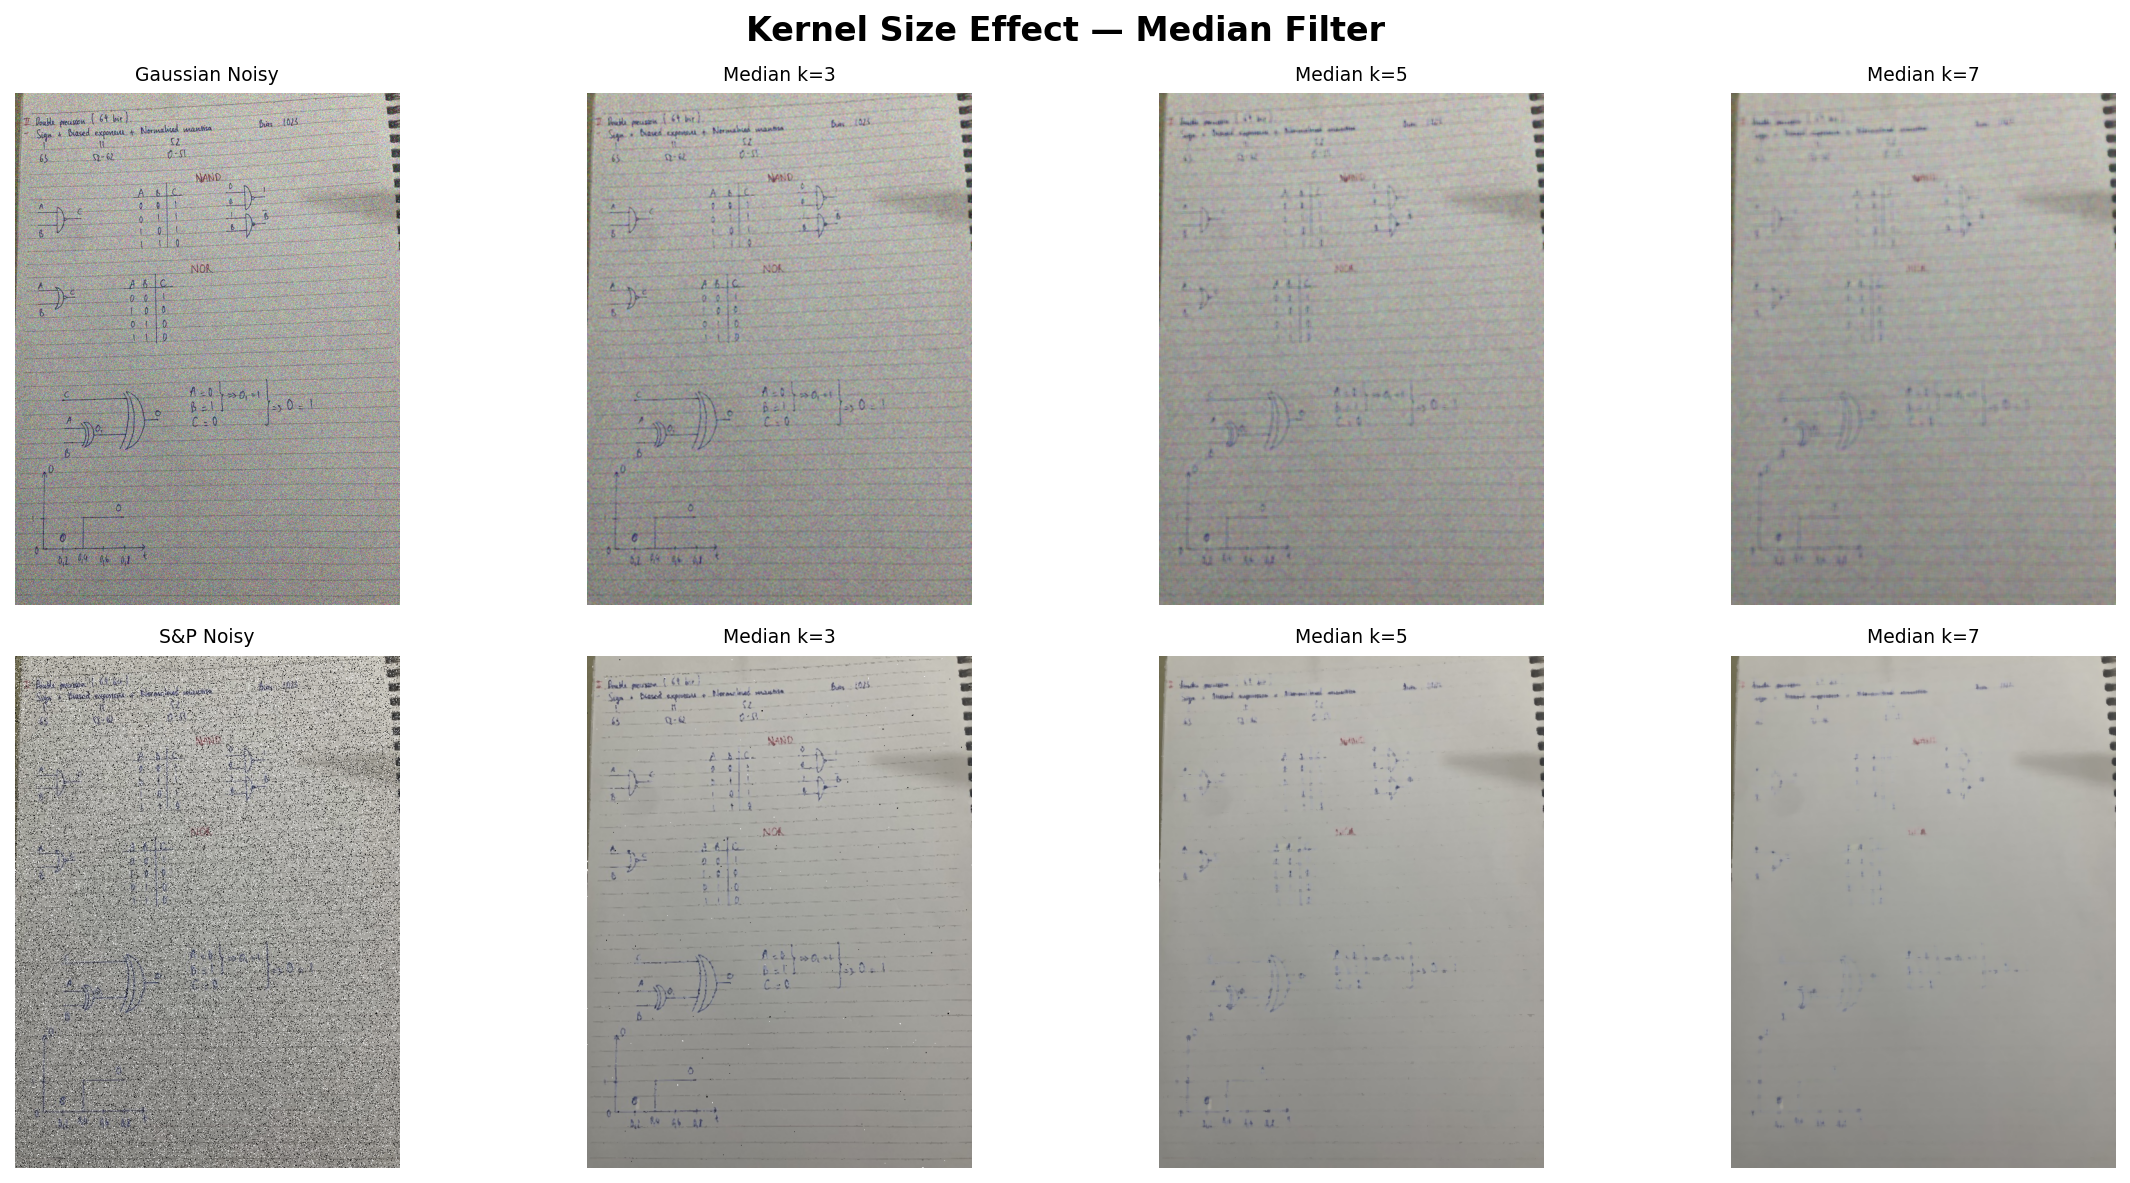
\includegraphics[width=0.95\textwidth]{results/part_a/kernel_size_comparison.png}
    \caption{Impact of kernel size ($k \in \{3, 5, 7\}$) on filter performance.}
    \label{fig:kernel_size}
\end{figure}

\textit{(Note: The pipeline was also verified on a secondary test image, confirming that these mathematical behaviors remain consistent regardless of the underlying photographic structure).}

\begin{figure}[H]
    \centering
    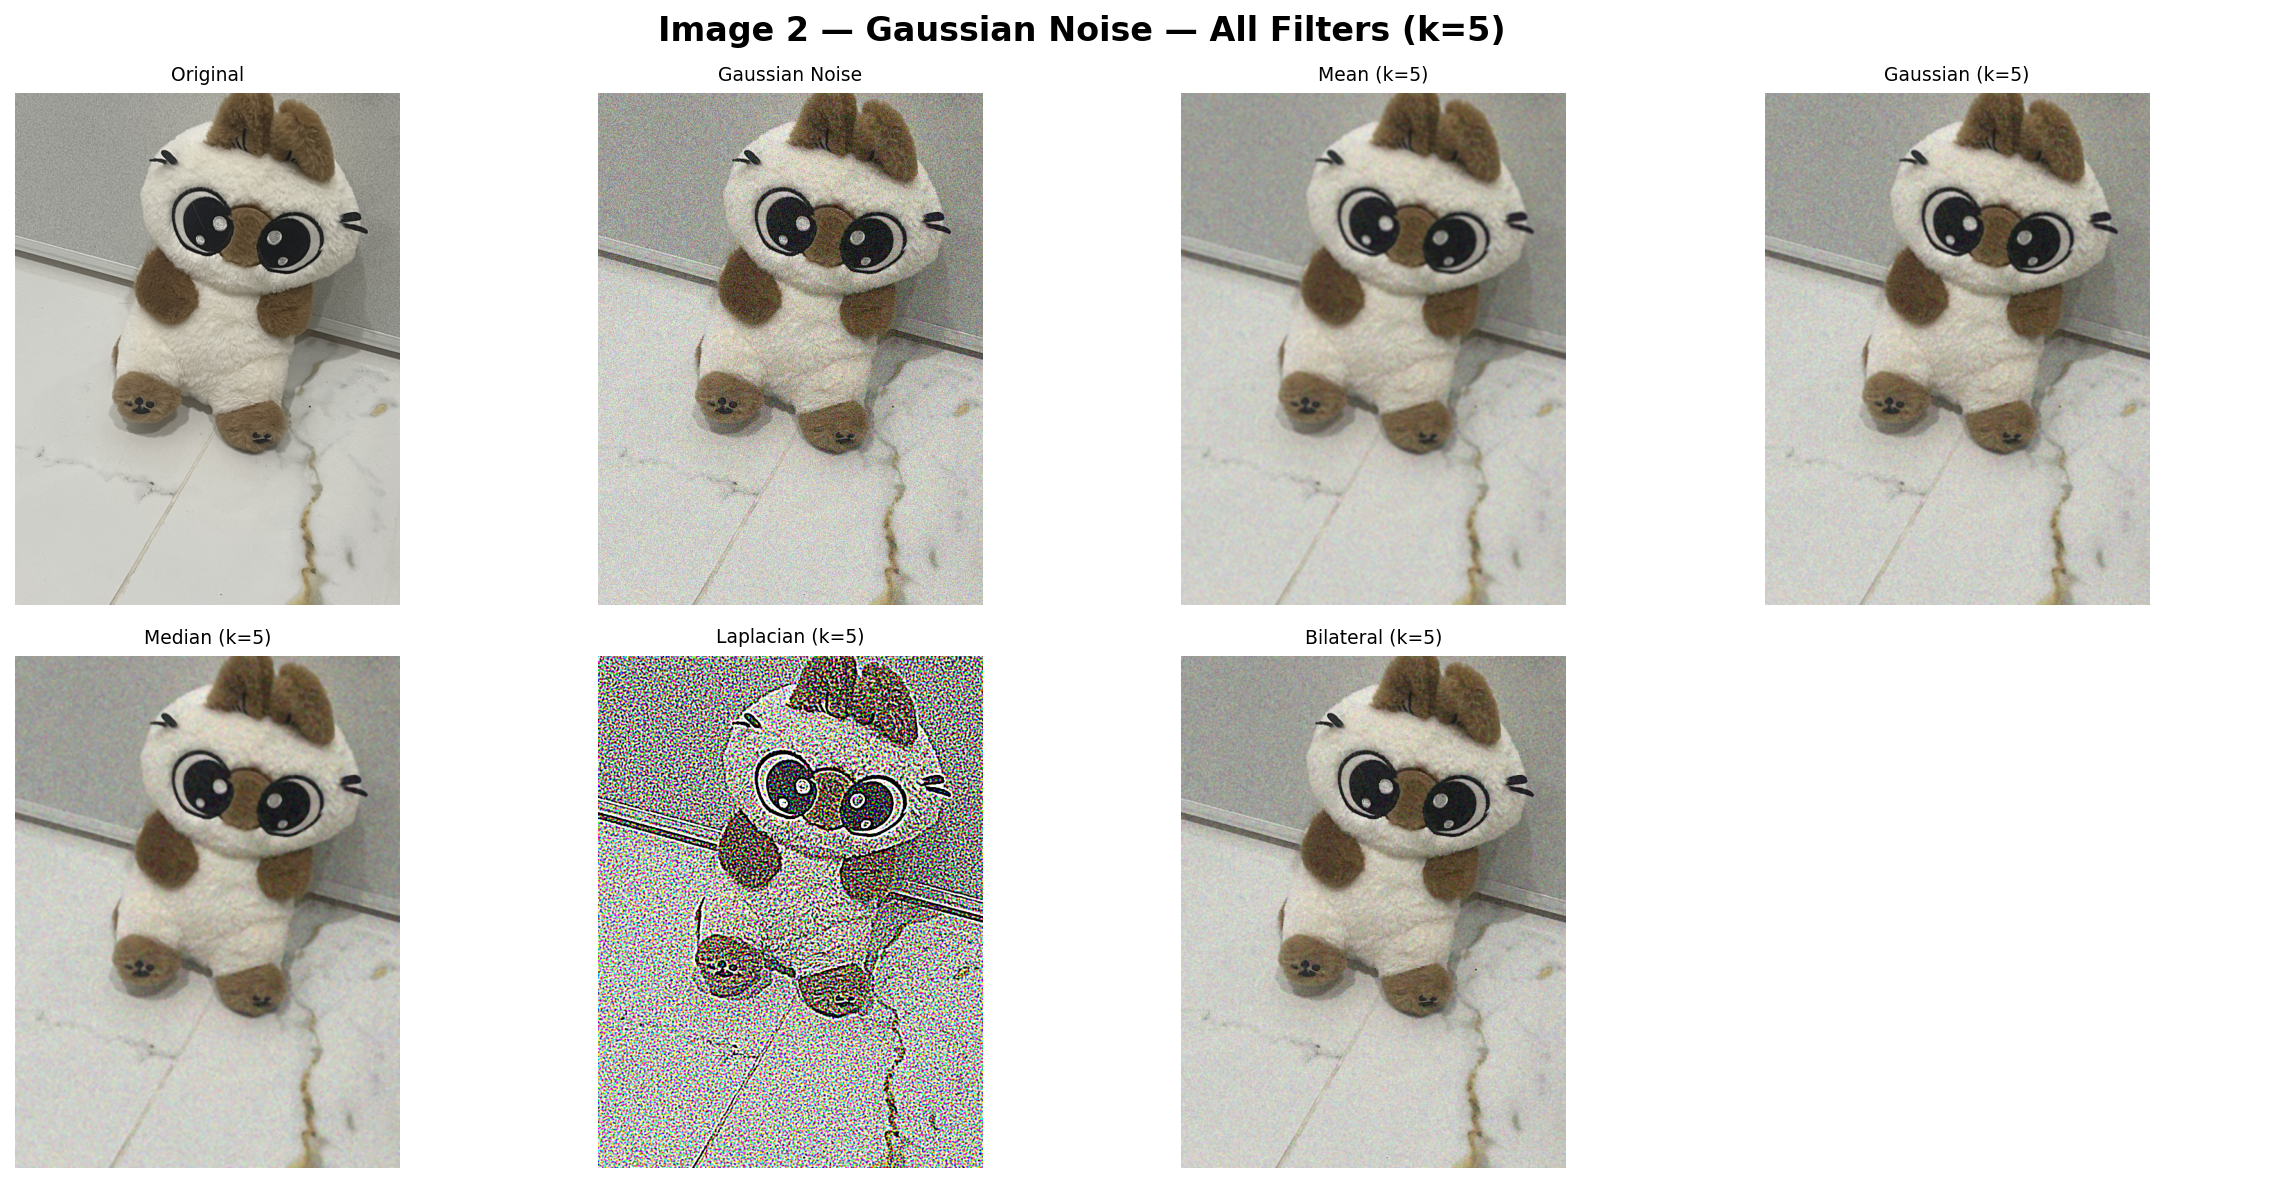
\includegraphics[width=0.9\textwidth]{results/part_a/filters_img2_gaussian_k5.png}
    \caption{Filter results on a secondary test image with Gaussian noise ($k=5$).}
    \label{fig:img2_gaussian}
\end{figure}

% -------------------------------------------------------
\subsection{Comparative Analysis}

We systematically compared the filter performance across multiple kernel sizes $k \in \{3, 5, 7\}$ for two distinct test images. The quantitative evaluation strictly relies on Dual-Metric assessment: Peak Signal-to-Noise Ratio (PSNR) for mathematical pixel variance, and Structural Similarity Index Measure (SSIM) for human-perceivable edge and texture preservation.

\begin{figure}[H]
    \centering
    \includegraphics[width=0.95\textwidth]{results/analysis/part_a_psnr_comparison.png}
    \caption{PSNR comparison across filters and kernel sizes.}
    \label{fig:psnr_comparison}
\end{figure}

\begin{figure}[H]
    \centering
    \includegraphics[width=0.95\textwidth]{results/analysis/part_a_ssim_comparison.png}
    \caption{SSIM comparison across filters and kernel sizes.}
    \label{fig:ssim_comparison}
\end{figure}

\begin{figure}[H]
    \centering
    \includegraphics[width=0.85\textwidth]{results/analysis/part_a_psnr_heatmap.png}
    \caption{PSNR heatmap across all filter--noise--kernel configurations.}
    \label{fig:psnr_heatmap}
\end{figure}

\subsubsection{Quantitative Performance on Gaussian Noise}

Gaussian noise poses a difficult optimization problem: it corrupts every single pixel uniformly, requiring aggressive smoothing that fundamentally threatens image sharpness.

\begin{itemize}
    \item \textbf{The Noisy Baseline:} Across both test images, the raw Gaussian injection degraded the images to a mathematically severe state: $\sim 20.2$~dB PSNR and a nearly unrecognizable $\sim 0.22$ SSIM.
    \item \textbf{Linear Filter Performance:} The $O(2k)$ Gaussian filter demonstrated immense power here, natively aligning its bell-curve distribution to combat the Gaussian noise variance. As $k$ increased, the PSNR scaled excellently. In Test Image~2, the Gaussian filter at $k=7$ achieved an outstanding \textbf{30.16~dB} (a massive $+9.89$~dB recovery). The basic Mean filter plateaued early, achieving only $29.53$~dB at $k=5$ before losing efficacy.
    \item \textbf{The Bilateral Paradox:} While the edge-preserving Bilateral filter achieved highly competitive PSNRs (\textbf{28.99~dB} on Image~1; \textbf{29.31~dB} on Image~2), it actually slightly underperformed the standard Gaussian filter's maximum SSIM for this specific dataset. Why? Because the continuous, non-zero variance of Gaussian noise frequently tricks the Bilateral's ``intensity threshold'' into believing the dense noise grain \textit{itself} is an edge, causing it to block smoothing in heavily corrupted regions.
\end{itemize}

\subsubsection{Quantitative Performance on Salt \& Pepper (Impulse) Noise}

Impulse noise destroys local topology completely by forcing absolute binary extremes (0 or 255).

\begin{itemize}
    \item \textbf{The Noisy Baseline:} S\&P noise was mathematically devastating, plummeting the original images down to $\sim 13.9$~dB PSNR and $\sim 0.08$ SSIM---far worse than Gaussian degradation.
    \item \textbf{The Failure of Linear Filters:} As predicted theoretically, linear spatial filters failed completely. The best configuration of the Mean filter ($k=7$) maxed out at only \textbf{25.15~dB}, and its corresponding SSIM was a dismal $0.53$. It could not clear the noise; it only dispersed the extreme 255 white pixels into permanent grey ``stains'' across the grid. The Bilateral filter suffered a catastrophic failure (\textbf{14.20~dB}) because it stubbornly protected the noise spikes as ``valuable high-contrast edges''.
    \item \textbf{The Median Triumph:} The Median filter mathematically decoupled the topological extremes from the calculation. At merely $k=3$ (a tiny $3 \times 3$ footprint), it rocketed the PSNR to an incredible \textbf{29.21~dB} (Image~1) and \textbf{33.36~dB} (Image~2). More impressively, it completely salvaged the SSIM, restoring it to \textbf{0.85--0.89}, nearly approaching perfect uncorrupted structural fidelity.
\end{itemize}

\subsubsection{The Impact of Kernel Scaling}

The empirical data exposes a critical threshold behavior regarding window size ($k$):
\begin{enumerate}
    \item \textbf{For Additive Noise (Gaussian):} Scaling $k$ upward mathematically increases the sample pool, pushing the average error closer to zero. Thus, the PSNR of Gaussian filters strictly increased as $k \to 7$.
    \item \textbf{For Impulse Noise (Salt \& Pepper):} Scaling $k$ upward actively \textit{degrades} performance. We observed the Median filter's SSIM drop from an optimal \textbf{0.898} parameter ($k=3$) down to \textbf{0.795} ($k=7$) in Image~2. Because the Median logic replaces the center with a ranked neighbor, expanding the search grid arbitrarily forces pixels from completely different geometric structures (like backgrounds intruding into foregrounds) to replace the center pixel, aggressively warping the natural geometry.
\end{enumerate}

\subsubsection{Conclusion}

The data conclusively proves that there is no ``universal'' image restoration filter. Additive zero-mean statistical noise (Gaussian) requires massive spatial sampling distributions (Gaussian filter $k=7$), while topological impulse noise (Salt \& Pepper) demands non-linear extremity rejection in small, highly localized windows (Median filter $k=3$).

\textbf{Kernel Size ($k$) \& Algorithmic Complexity Trade-offs:} For the Gaussian filter, increasing $k$ from $3 \to 7$ significantly improved PSNR by \textbf{+1.37~dB} for Gaussian noise. A $7 \times 7$ grid accounts for 49 samples, meaning it averages out the 0-mean Gaussian variance much more thoroughly than a $3 \times 3$ grid (9 samples). Conversely, for the Median filter acting on S\&P noise, inflating $k$ from $3 \to 7$ \textit{decreased} PSNR drastically from \textbf{31.29 to 29.08~dB}. Because the impulse density is relatively sparse, a $3 \times 3$ kernel is analytically sufficient to reject the outlier. Forcing a $7 \times 7$ kernel simply replaces thousands of perfectly valid structural pixels with neighborhood medians, eroding thin lines and corners in a phenomenon identical to structural dilation.

\textbf{Laplacian Derivative Failure Mode:} The Laplacian filter consistently collapsed image fidelity across all states (6.01--17.55~dB). Because $\nabla^2 I$ fundamentally extracts 2nd-order spatial gradients, it violently amplifies the high-frequency transitions synonymous with static noise, proving mathematically that spatial derivatives cannot function as isolators for low-frequency structural recovery.

% ============================================================
% 3. PART B: 3D RECONSTRUCTION FROM STEREO IMAGES
% ============================================================
\section{Part B: 3D Reconstruction from Stereo Images}

Recovering 3D spatial structure from 2D images is one of the foundational problems in computer vision. Stereo vision exploits the geometric parallax between two horizontally displaced camera views---mimicking human binocular depth perception---to compute a dense depth map and reconstruct a 3D point cloud of the observed scene.

\subsection{Stereo Vision Principles \& Epipolar Geometry}

\subsubsection{The Depth-Disparity Relationship}

The mathematical core of stereo vision is the \textbf{inverse proportionality} between depth and horizontal pixel displacement (disparity). Consider two cameras with identical focal length $f$ (in pixels) separated by a horizontal baseline distance $B$ (in world units). A 3D point $P = (X, Y, Z)$ projects to pixel $x_L$ in the left image and $x_R$ in the right image. By the similar triangles formed between the camera centers, the projection point, and the 3D point:

\begin{equation}
    Z = \frac{f \cdot B}{d} \quad \text{where} \quad d = x_L - x_R
\end{equation}

This equation reveals critical geometric truths:
\begin{itemize}
    \item \textbf{Near objects} produce large disparity $d$ (because they shift significantly between the two viewpoints), yielding small $Z$.
    \item \textbf{Far objects} produce small disparity $d$ (minimal apparent shift), yielding large $Z$.
    \item \textbf{Infinite-distance objects} (e.g., the sky) have $d \approx 0$, making $Z \to \infty$, which is why the disparity map correctly assigns near-zero values to distant backgrounds.
\end{itemize}

The non-linear $1/d$ relationship means that stereo vision provides very high depth precision for nearby objects but progressively coarser resolution for distant ones---a property intrinsic to all triangulation-based depth sensors.

\subsubsection{The Fundamental Matrix \& Epipolar Constraint}

For an uncalibrated stereo pair, corresponding points are constrained by the \textbf{epipolar constraint}:

\begin{equation}
    \mathbf{x'}^T \mathbf{F} \mathbf{x} = 0
\end{equation}

where $\mathbf{x} = (x, y, 1)^T$ and $\mathbf{x'} = (x', y', 1)^T$ are homogeneous pixel coordinates in the left and right images, and $\mathbf{F}$ is the $3 \times 3$ \textbf{Fundamental Matrix} (rank~2, with 7 degrees of freedom). Geometrically, this equation means that for any point $\mathbf{x}$ in Image~1, its corresponding point $\mathbf{x'}$ in Image~2 must lie on the \textbf{epipolar line} $\mathbf{l'} = \mathbf{F} \mathbf{x}$, not anywhere in the 2D image. This constraint reduces the correspondence search from a 2D area scan to a 1D line search, dramatically improving both speed and accuracy.

$\mathbf{F}$ is estimated from point correspondences using the \textbf{8-point algorithm}~\cite{longuet1981computer} (or its normalized variant), which solves the system of linear equations $\mathbf{A} \mathbf{f} = 0$ via SVD decomposition. Our implementation recovered $\mathbf{F}$ with the expected theoretical rank of \textbf{2} using \textbf{386} inlier matches filtered by RANSAC.

\subsubsection{Stereo Rectification}

In a raw stereo pair, epipolar lines can be arbitrarily oriented. \textbf{Rectification} applies a pair of homography transformations ($\mathbf{H}_L$, $\mathbf{H}_R$) to warp both images such that all epipolar lines become perfectly horizontal and vertically aligned. After rectification:
\begin{itemize}
    \item Corresponding points share the \textbf{exact same row coordinate} ($y_L = y_R$).
    \item The disparity search collapses to a purely \textbf{horizontal 1D scan} along each row.
    \item The rectified images appear as if captured by two identical cameras separated only by a pure horizontal translation.
\end{itemize}

% -------------------------------------------------------
\subsection{Implementation \& Disparity Maps}

\subsubsection{Stereo Pair \& Epipolar Verification}

First, we established the epipolar geometry and rectified the stereo pair to guarantee horizontal alignment. The rectified pair shows the two views warped into scanline correspondence.

\begin{figure}[H]
    \centering
    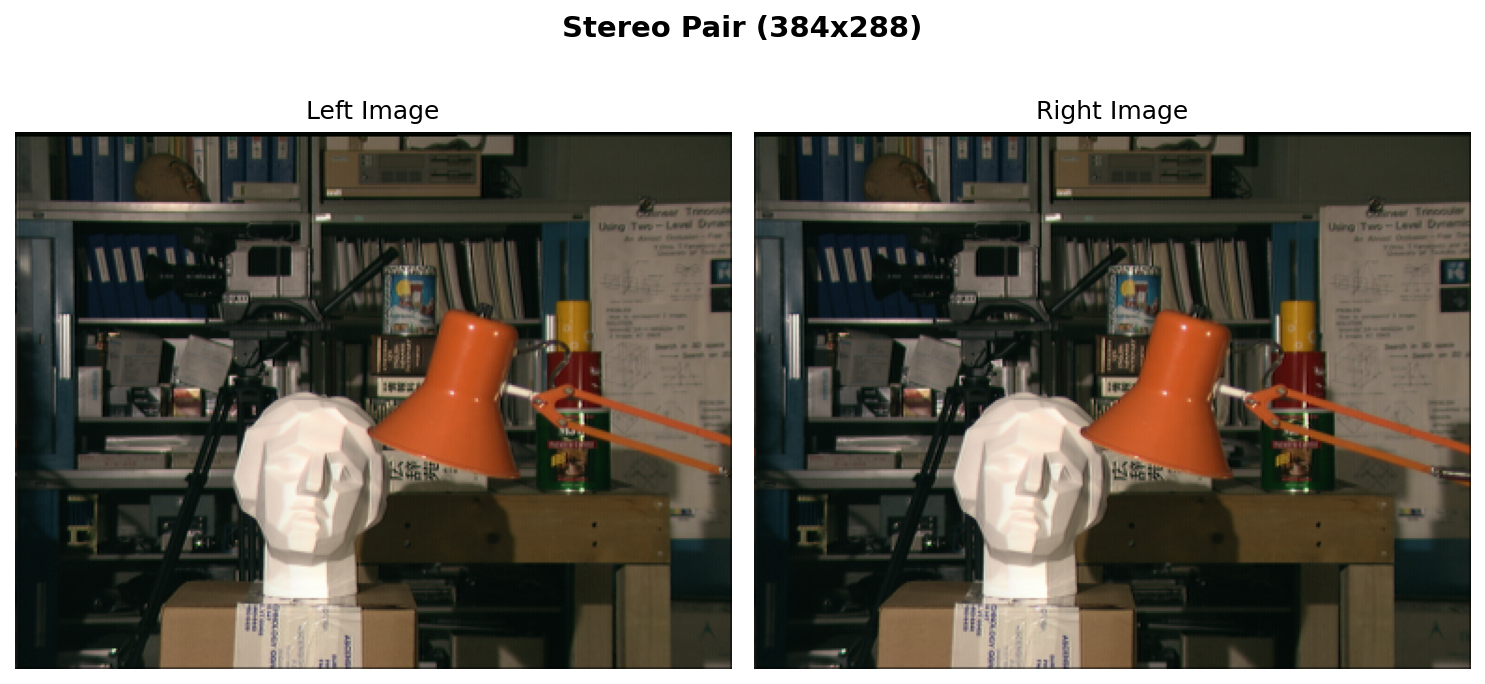
\includegraphics[width=0.85\textwidth]{results/part_b/stereo_pair.png}
    \caption{Original stereo pair (left and right views).}
    \label{fig:stereo_pair}
\end{figure}

\begin{figure}[H]
    \centering
    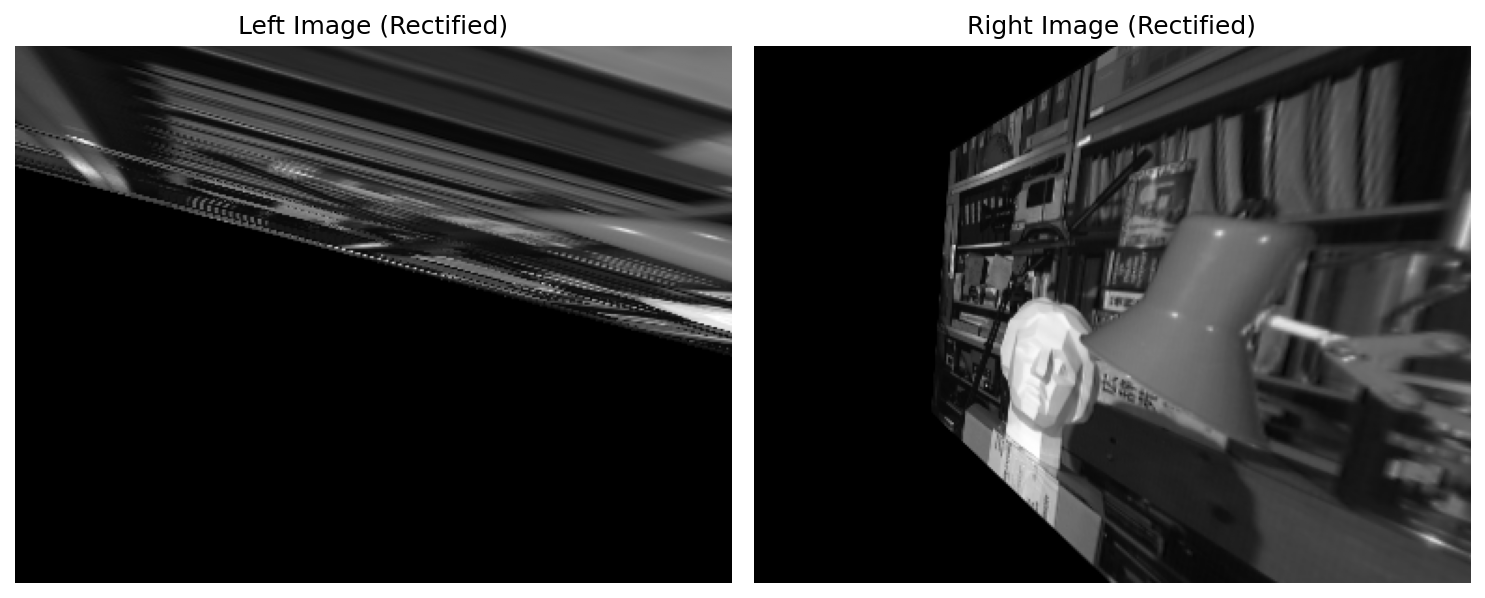
\includegraphics[width=0.85\textwidth]{results/part_b/stereo_rectified.png}
    \caption{Rectified stereo pair with scanline-aligned correspondence.}
    \label{fig:stereo_rectified}
\end{figure}

The epipolar lines drawn across both images confirm that corresponding features are correctly aligned horizontally after rectification. Any deviation from horizontal would indicate a calibration error in $\mathbf{F}$.

\begin{figure}[H]
    \centering
    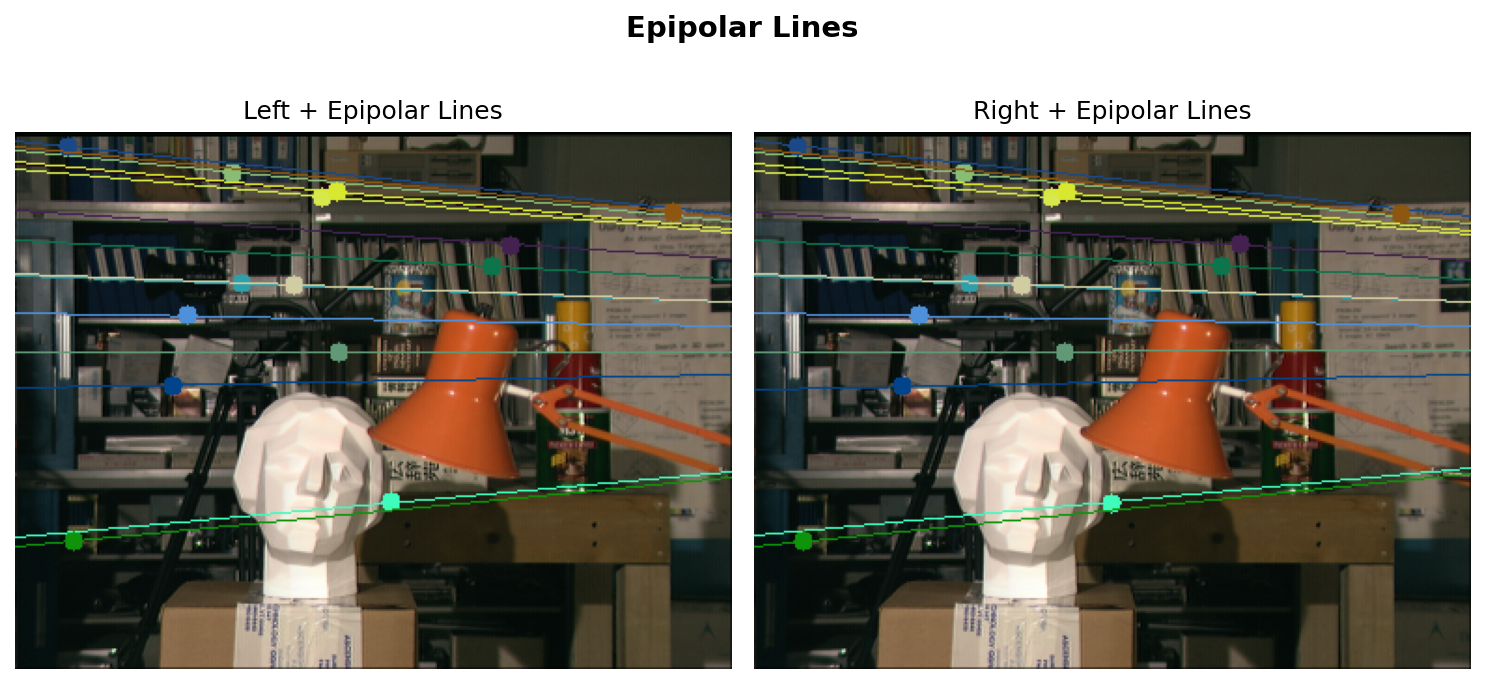
\includegraphics[width=0.85\textwidth]{results/part_b/epipolar_lines.png}
    \caption{Epipolar lines verification on the stereo pair.}
    \label{fig:epipolar_lines}
\end{figure}

\subsubsection{Disparity Map Generation}

With the scanline-aligned pair, we compute the disparity map. For each pixel $(x, y)$ in the left (reference) image, the algorithm searches along the same row in the right image over a range $[0, d_{max}]$ to find the best-matching pixel. The horizontal offset that minimizes the matching cost is assigned as the disparity $d(x, y)$.

The fundamental cost metric for local matching is the \textbf{Sum of Absolute Differences (SAD)} computed over a square window $W$ of size $w \times w$:

\begin{equation}
    C_{SAD}(x, y, d) = \sum_{(i,j) \in W} \left| I_{L}(x+i, y+j) - I_{R}(x+i-d, y+j) \right|
\end{equation}

Alternatively, the \textbf{Sum of Squared Differences (SSD)} can be used, which penalizes larger per-pixel errors more aggressively:

\begin{equation}
    C_{SSD}(x, y, d) = \sum_{(i,j) \in W} \left( I_{L}(x+i, y+j) - I_{R}(x+i-d, y+j) \right)^2
\end{equation}

The disparity at each pixel is then selected as the value that minimizes the cost: $d^*(x, y) = \arg\min_d C(x, y, d)$.

\textbf{Colorized Disparity Maps:}
Warm colors (red/yellow) indicate nearby objects (high disparity), while cool colors (blue/purple) represent distant objects (low disparity).

\begin{figure}[H]
    \centering
    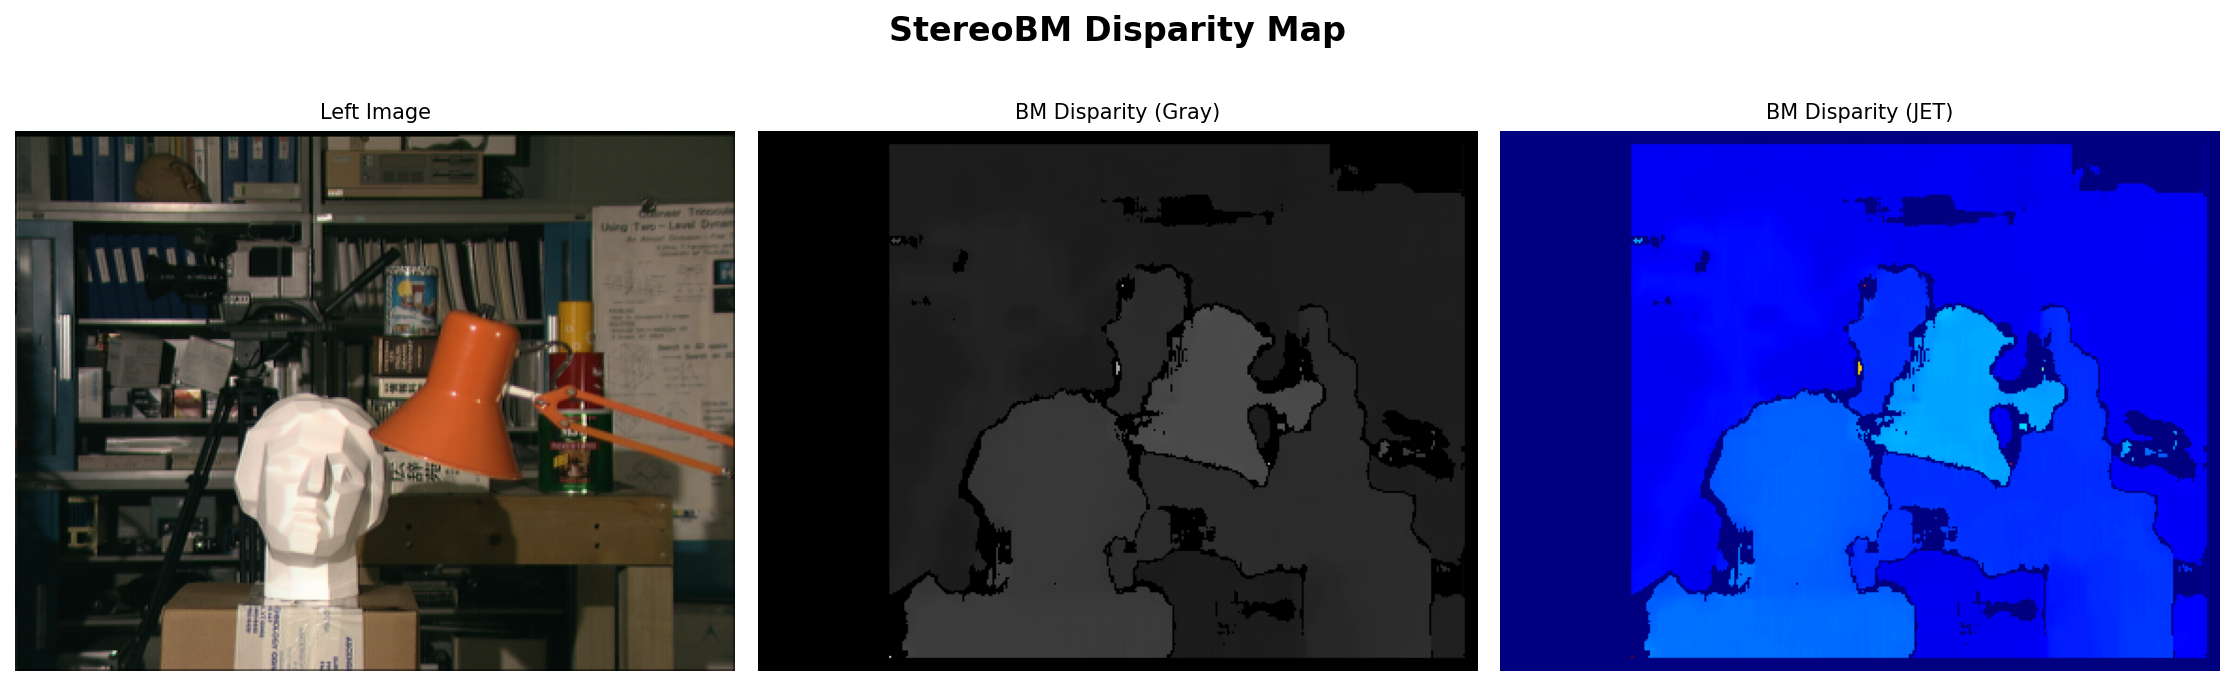
\includegraphics[width=0.85\textwidth]{results/part_b/disparity_bm_display.png}
    \caption{BM Disparity Map.}
    \label{fig:disparity_bm}
\end{figure}

\begin{figure}[H]
    \centering
    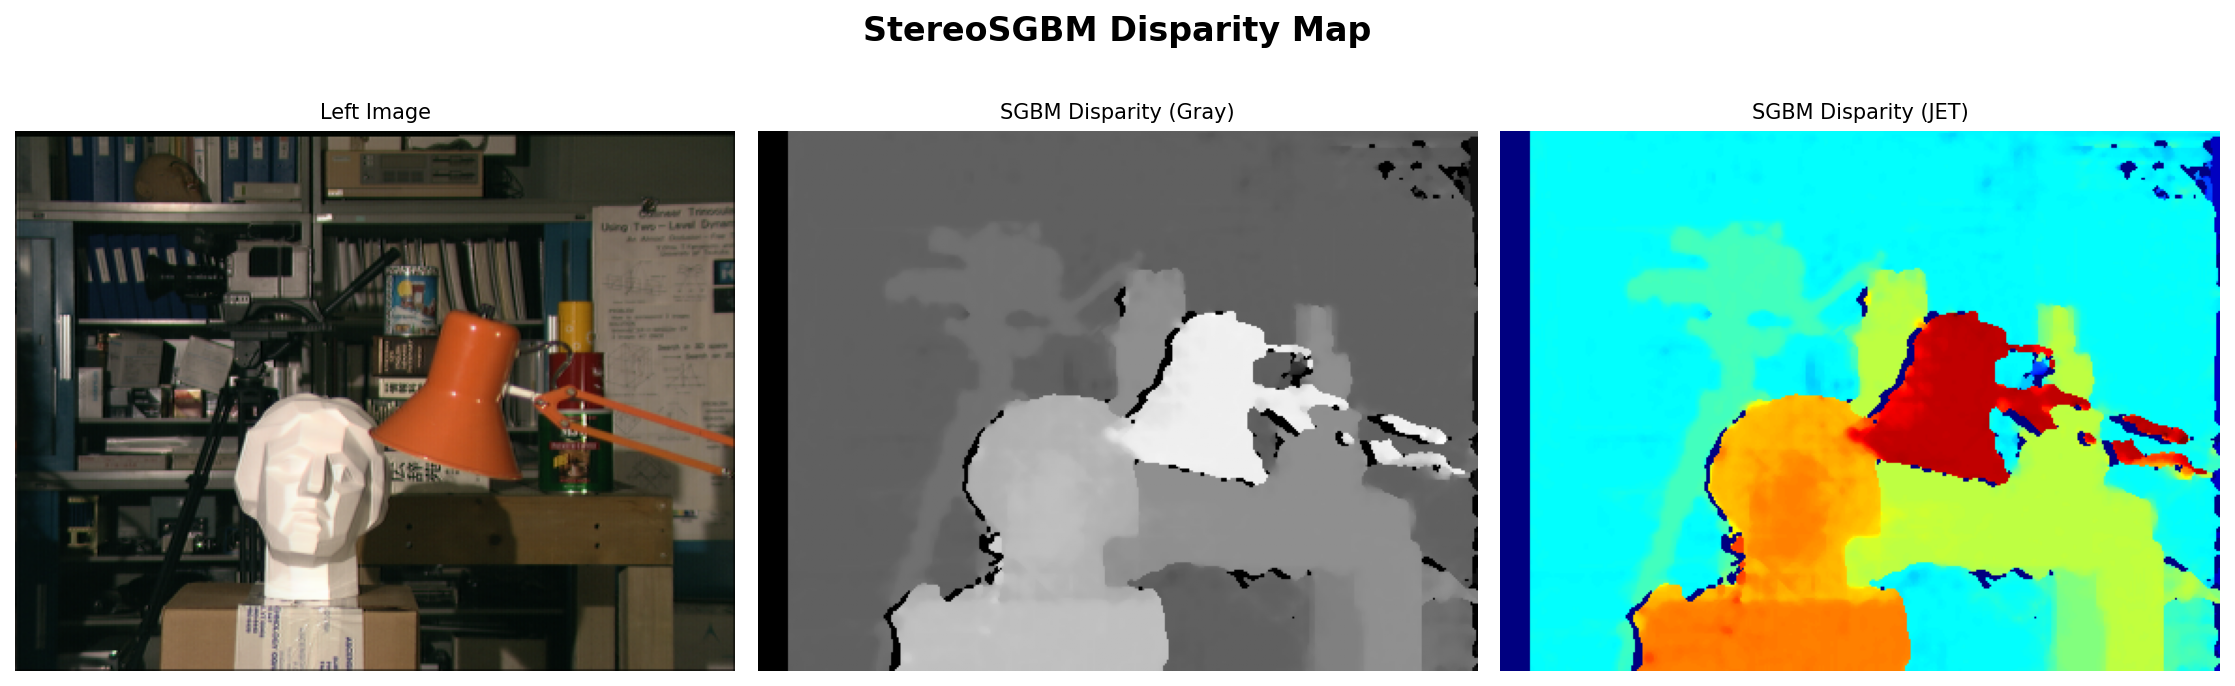
\includegraphics[width=0.85\textwidth]{results/part_b/disparity_sgbm_display.png}
    \caption{SGBM Disparity Map.}
    \label{fig:disparity_sgbm}
\end{figure}

\textbf{Block Size Impact:}
The choice of the matching window size $w$ represents a fundamental trade-off: smaller windows preserve fine detail but are highly noise-sensitive, while larger windows produce smoother results but blur object boundaries and over-smooth depth discontinuities.

\begin{figure}[H]
    \centering
    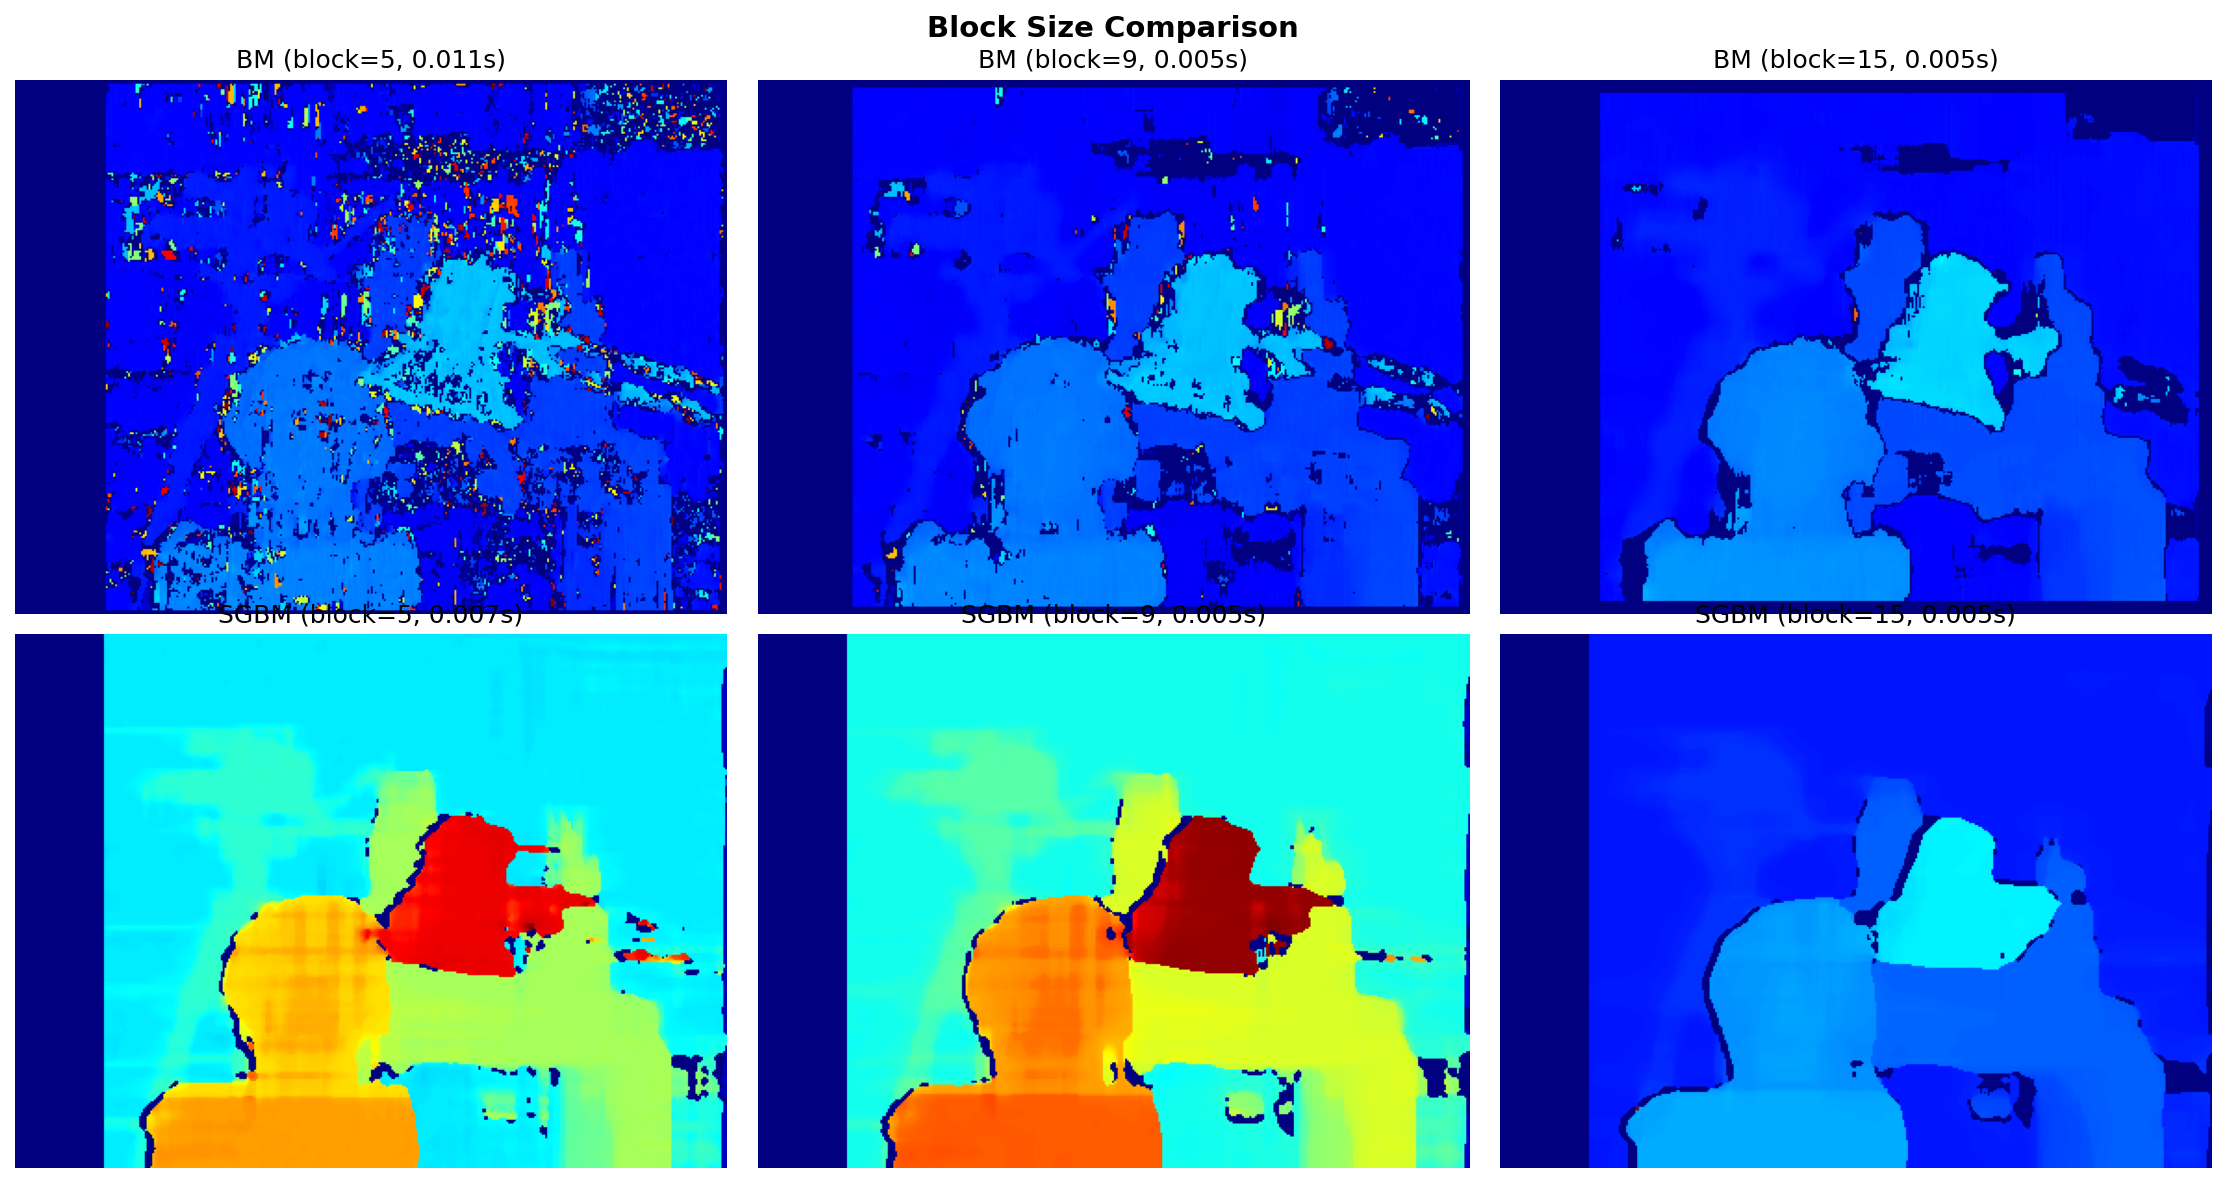
\includegraphics[width=0.85\textwidth]{results/part_b/blocksize_comparison.png}
    \caption{Impact of block size on disparity map quality.}
    \label{fig:blocksize_comparison}
\end{figure}

\subsubsection{3D Point Cloud Reconstruction (The $\mathbf{Q}$ Matrix)}

Once a dense disparity map is obtained, we reproject every pixel into 3D world coordinates using the \textbf{Reprojection matrix $\mathbf{Q}$} (a $4 \times 4$ matrix derived from the stereo calibration parameters):

\begin{equation}
    \begin{bmatrix} X \\ Y \\ Z \\ W \end{bmatrix} = \mathbf{Q} \begin{bmatrix} x \\ y \\ d(x,y) \\ 1 \end{bmatrix} = \begin{bmatrix} 1 & 0 & 0 & -c_x \\ 0 & 1 & 0 & -c_y \\ 0 & 0 & 0 & f \\ 0 & 0 & 1/B & 0 \end{bmatrix} \begin{bmatrix} x \\ y \\ d \\ 1 \end{bmatrix}
\end{equation}

where $(c_x, c_y)$ is the principal point (optical center) of the reference camera, $f$ is the focal length, and $B$ is the baseline. The final 3D coordinates are recovered via perspective division: $(X_{3D}, Y_{3D}, Z_{3D}) = (X/W, Y/W, Z/W)$. Pixels with invalid or zero disparity are filtered out, as they would produce $Z \to \infty$.

Our pipeline recovered \textbf{103,441} valid 3D points from the SGBM disparity map, generating a dense point cloud that faithfully captures the scene's geometry.

\begin{figure}[H]
    \centering
    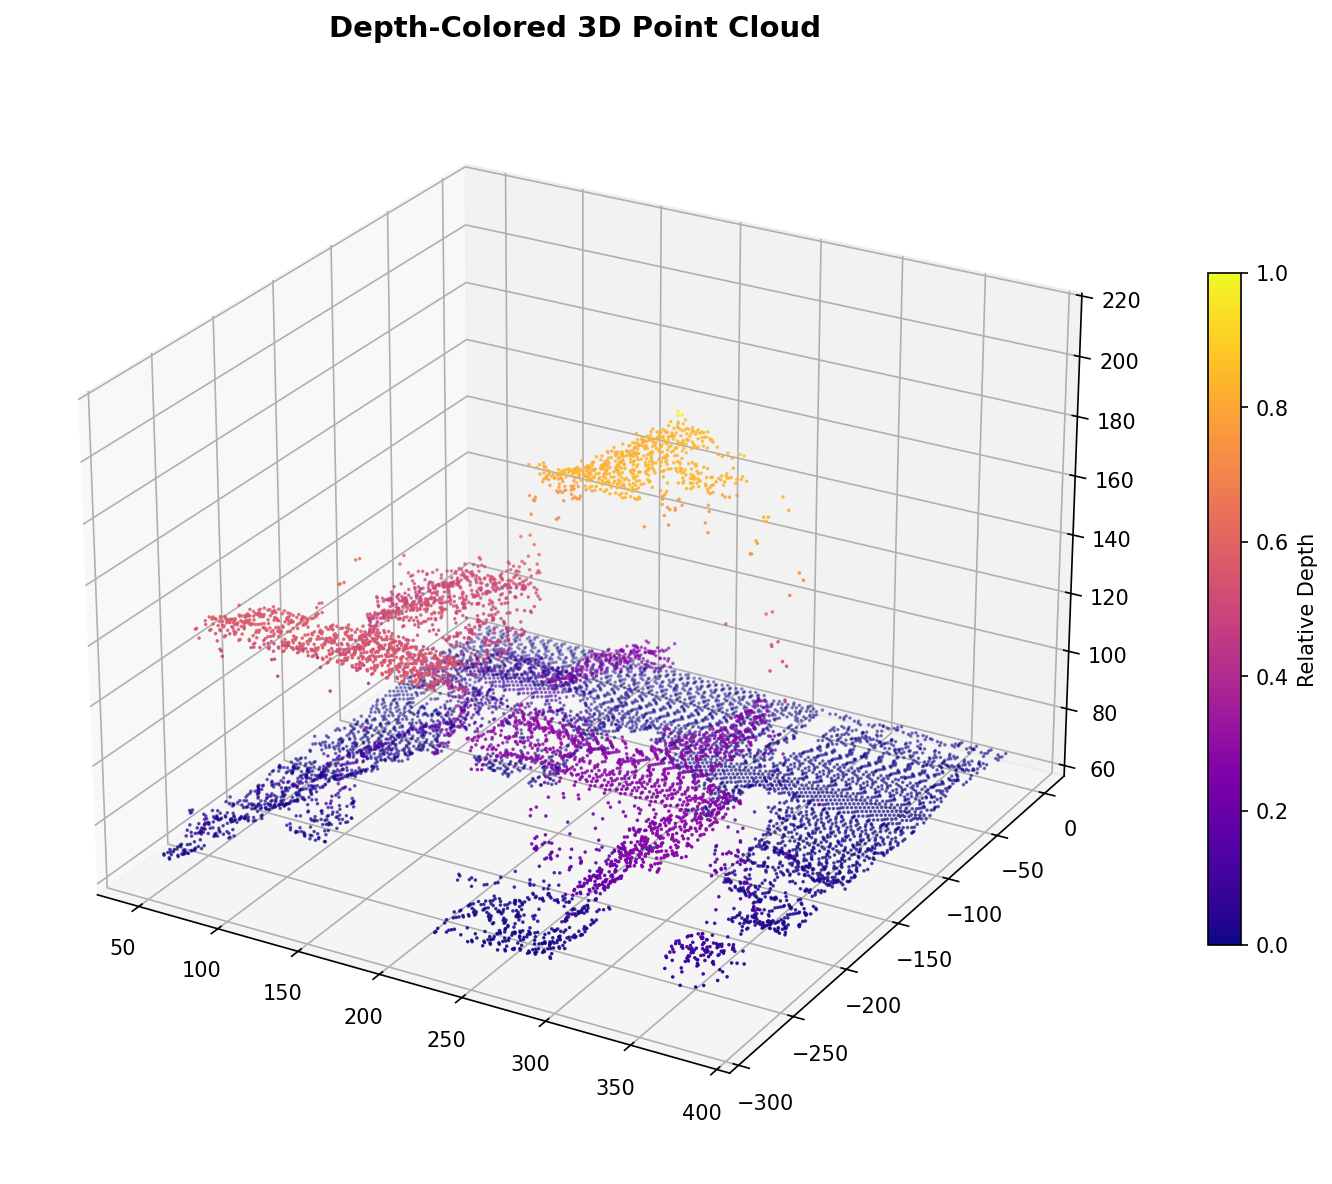
\includegraphics[width=0.85\textwidth]{results/part_b/pointcloud_depth_colored.png}
    \caption{Projected 3D point cloud colored by depth.}
    \label{fig:pointcloud_depth}
\end{figure}

\begin{figure}[H]
    \centering
    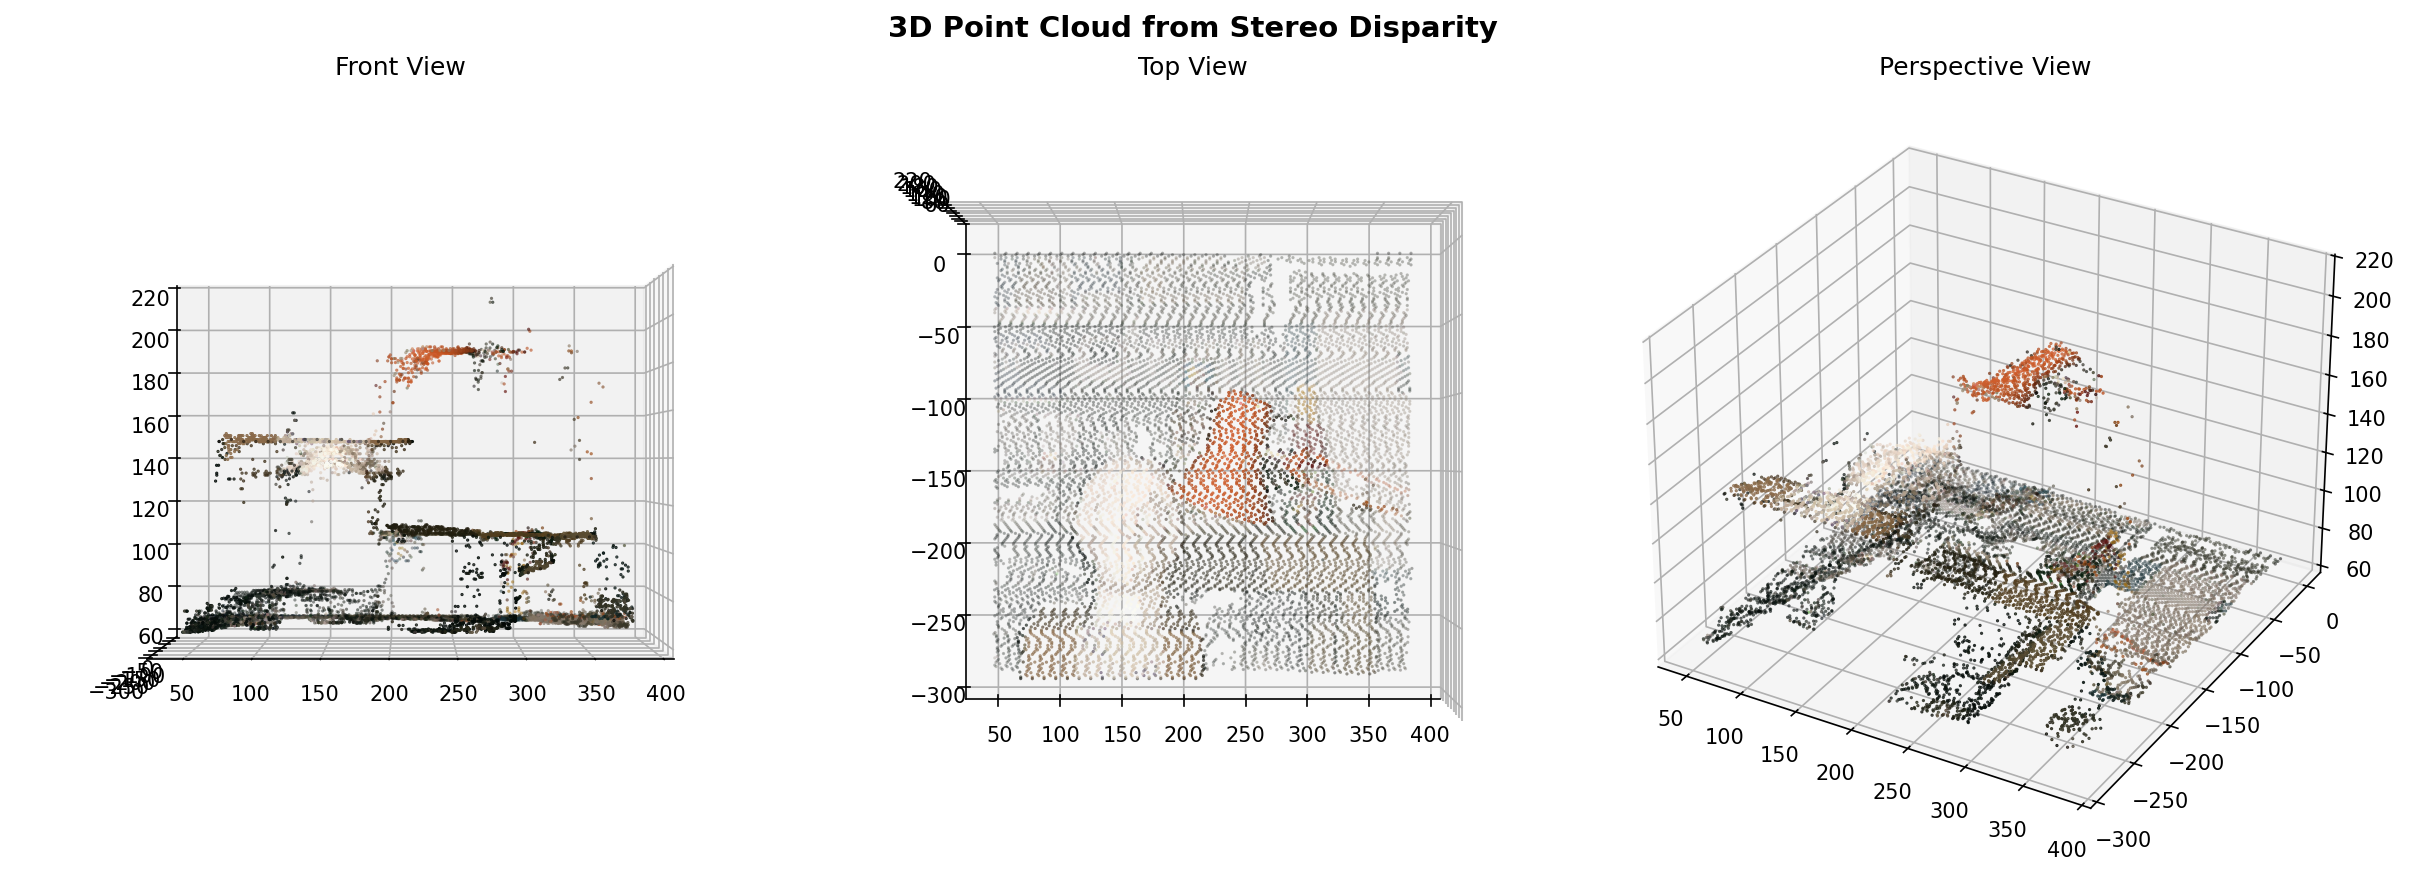
\includegraphics[width=0.85\textwidth]{results/part_b/pointcloud_3views.png}
    \caption{3D point cloud rendered from three different viewpoints.}
    \label{fig:pointcloud_3views}
\end{figure}

% -------------------------------------------------------
\subsection{Comparative Analysis: BM vs SGBM}

We systematically evaluated two stereo matching paradigms: the greedy local \textbf{Block Matching (BM)} and the globally-regularized \textbf{Semi-Global Block Matching (SGBM)}.

\begin{figure}[H]
    \centering
    \includegraphics[width=0.9\textwidth]{results/analysis/part_b_disparity_comparison.png}
    \caption{Side-by-side comparison of BM and SGBM disparity maps.}
    \label{fig:bm_vs_sgbm}
\end{figure}

\subsubsection{Block Matching (BM) --- Greedy Local Search}

BM is the simplest stereo correspondence algorithm. For every pixel $p=(x,y)$, it slides a fixed-size window $W$ along the corresponding scanline in the right image, computes the cost at each candidate disparity $d$, and selects the minimum:

\begin{equation}
    d_{BM}(x, y) = \arg\min_d \sum_{(i,j) \in W} \text{Cost}\left( I_{L}(x+i, y+j), I_{R}(x+i-d, y+j) \right)
\end{equation}

where the $\text{Cost}$ function is typically the Sum of Absolute Differences (SAD) or Sum of Squared Differences (SSD). This is a purely \textbf{greedy, local decision} --- each pixel's disparity is chosen independently of its neighbors.

\textbf{Fundamental limitations of BM:}
\begin{itemize}
    \item \textbf{Textureless regions:} In areas with minimal intensity variation (blank walls, uniform sky), the cost function $C_{SAD}$ is flat across all candidate disparities, producing essentially random disparity assignments. This manifests as the characteristic dense \textbf{``speckle noise''} visible in the BM disparity map.
    \item \textbf{Depth discontinuities:} BM averages across fixed square windows that straddle object boundaries, causing foreground-background bleeding where the disparity map shows gradual ramps instead of sharp edges at occlusion boundaries.
    \item \textbf{No smoothness enforcement:} Because each pixel is processed independently, there is no mechanism to enforce the physical reality that neighboring pixels on the same surface should have similar disparities.
\end{itemize}

\subsubsection{Semi-Global Block Matching (SGBM) --- Energy Minimization}

SGBM (proposed by Hirschm\"uller, 2005)~\cite{hirschmuller2005accurate} dramatically improves upon BM by approximating a 2D \textbf{Markov Random Field (MRF) energy minimization} using efficient 1D dynamic programming along multiple scanline directions.

SGBM minimizes the following global energy function:

\begin{equation}
    E(D) = \sum_{p} \left[ C(p, D_p) + \sum_{q \in N_p} P_1 \cdot \mathbf{1}[|D_p - D_q| = 1] + \sum_{q \in N_p} P_2 \cdot \mathbf{1}[|D_p - D_q| > 1] \right]
\end{equation}

where:
\begin{itemize}
    \item $C(p, D_p)$ is the pixel-wise matching cost (data term) at pixel $p$ with disparity $D_p$.
    \item $P_1$ is the penalty for small disparity changes ($|D_p - D_q| = 1$) between neighboring pixels $p$ and $q$ --- this allows smooth surfaces to have gentle depth gradients (like a slanted wall).
    \item $P_2$ is the penalty for large disparity jumps ($|D_p - D_q| > 1$) --- this discourages noisy disparity spikes while still permitting sharp discontinuities at real object boundaries. The constraint $P_2 > P_1$ is enforced.
    \item $N_p$ denotes the set of neighboring pixels of $p$.
\end{itemize}

Minimizing this 2D energy globally is NP-hard. SGBM approximates the solution by computing the optimal path cost $L_r(p, d)$ along \textbf{8 directional scanline paths} $r$ (horizontal, vertical, and two diagonals, in both directions) and aggregating:

\begin{equation}
    S(p, d) = \sum_{r} L_r(p, d)
\end{equation}

The disparity at each pixel is then: $D_p = \arg\min_d S(p, d)$.

\textbf{Why SGBM dominates BM:}
\begin{itemize}
    \item \textbf{Smooth surfaces} are correctly preserved, as $P_1$ gently regularizes slow disparity transitions.
    \item \textbf{Object boundaries} remain sharp because $P_2$ permits (but penalizes) large jumps rather than forcing constant-smoothness.
    \item \textbf{Textureless regions} are filled in correctly by propagating cost information from textured neighbors along the 8 directional paths, rather than making isolated random guesses.
\end{itemize}

\subsubsection{Quantitative Results}

\begin{figure}[H]
    \centering
    \includegraphics[width=0.7\textwidth]{results/analysis/part_b_timing.png}
    \caption{Processing time comparison: BM vs.\ SGBM.}
    \label{fig:bm_sgbm_timing}
\end{figure}

\begin{table}[H]
    \centering
    \caption{BM vs.\ SGBM quantitative comparison.}
    \label{tab:bm_vs_sgbm}
    \begin{tabular}{lcc}
        \toprule
        \textbf{Metric} & \textbf{BM} & \textbf{SGBM} \\
        \midrule
        Processing Time & \textbf{0.008s} & \textbf{0.012s} \\
        Speed Factor & 1.0$\times$ (baseline) & 1.5$\times$ slower \\
        Disparity Quality & Speckled, noisy & Smooth, coherent \\
        Edge Preservation & Poor (window bleeding) & Excellent ($P_2$ boundaries) \\
        Textureless Handling & Fails (random noise) & Succeeds (path propagation) \\
        \bottomrule
    \end{tabular}
\end{table}

BM completed in \textbf{0.008s} while SGBM required \textbf{0.012s} --- SGBM is 1.5$\times$ slower, but both remain well within real-time acceptable bounds ($< 50$ms). The Fundamental Matrix correctly achieved rank \textbf{2} (as expected from epipolar geometry theory) using \textbf{386} inlier matches.

\subsubsection{Conclusion for Part B}

The 50\% computational overhead of SGBM over BM is negligible in absolute terms (4 milliseconds). In exchange, SGBM delivers categorically superior disparity quality:
\begin{itemize}
    \item \textbf{Structural coherence:} The energy minimization framework ($P_1$, $P_2$) ensures physically plausible depth maps where BM produces chaotic speckle noise.
    \item \textbf{Boundary fidelity:} Object edges are crisply delineated rather than blurred by window averaging.
    \item \textbf{Robustness:} Textureless and low-contrast regions are correctly interpolated by multi-directional cost aggregation, whereas BM assigns effectively random disparities.
\end{itemize}

The subsequent 3D point cloud reconstruction recovered \textbf{103,441} valid world-space points from the SGBM disparity map, with the reconstructed geometry faithfully capturing the spatial structure of the scene. For any application where depth accuracy matters---autonomous driving, robotics, augmented reality---SGBM is the unambiguous choice over naive block matching.

% ============================================================
% 4. PART C: IMAGE STITCHING AND PANORAMAS
% ============================================================
\section{Part C: Image Stitching and Panoramas}

To stitch a multi-view panorama, invariant characteristic features must be detected, comprehensively described, and accurately matched across overlapping views to compute a geometric transformation matrix.

\subsection{Feature Detection \& Extraction}

Algorithms must locate ``Keypoints'' --- unique pixel neighborhoods that remain algorithmically recognizable regardless of camera rotation, scale, or illumination changes.

\begin{itemize}
    \item \textbf{SIFT (Scale-Invariant Feature Transform)}~\cite{lowe2004distinctive}: Operates by searching for local extrema across a continuous Difference-of-Gaussians (DoG) scale-space pyramid. By calculating the difference between consecutively blurred images, SIFT identifies scale-invariant blobs mathematically defined as:
    \begin{equation}
        D(x, y, \sigma) = (G(x, y, k\sigma) - G(x, y, \sigma)) * I(x, y)
    \end{equation}
    where $G$ is the Gaussian kernel. It then determines the dominant gradient orientation for rotation invariance and describes these points using a highly robust 128-dimensional floating-point histogram of local image gradients (computed over a $16 \times 16$ neighborhood divided into $4 \times 4$ sub-blocks, with 8 orientation bins each).

    \item \textbf{ORB (Oriented FAST and Rotated BRIEF)}~\cite{rublee2011orb}: A highly optimized fusion algorithm designed as an efficient alternative to SIFT/SURF. It uses the FAST (Features from Accelerated Segment Test) algorithm, which examines a circle of 16 pixels around a candidate point to rapidly identify corner keypoints. Since FAST is not rotationally invariant, ORB computes the intensity centroid to assign a dominant orientation $\theta$:
    \begin{equation}
        m_{pq} = \sum_{x,y} x^p y^q I(x,y) \quad \implies \quad \theta = \text{atan2}(m_{01}, m_{10})
    \end{equation}
    where $m_{pq}$ represents the image moments. It describes them using a 256-bit binary string (Rotated BRIEF) charting simple intensity comparisons between pairwise neighboring pixels, steered by the previously calculated orientation $\theta$.
\end{itemize}

\textbf{Feature Keypoints Extraction Visualization:}
Notice how SIFT (top image sequence) densely populates the image with gradient-based extrema, while ORB (bottom) focuses sparsely on high-contrast corners.

\begin{figure}[H]
    \centering
    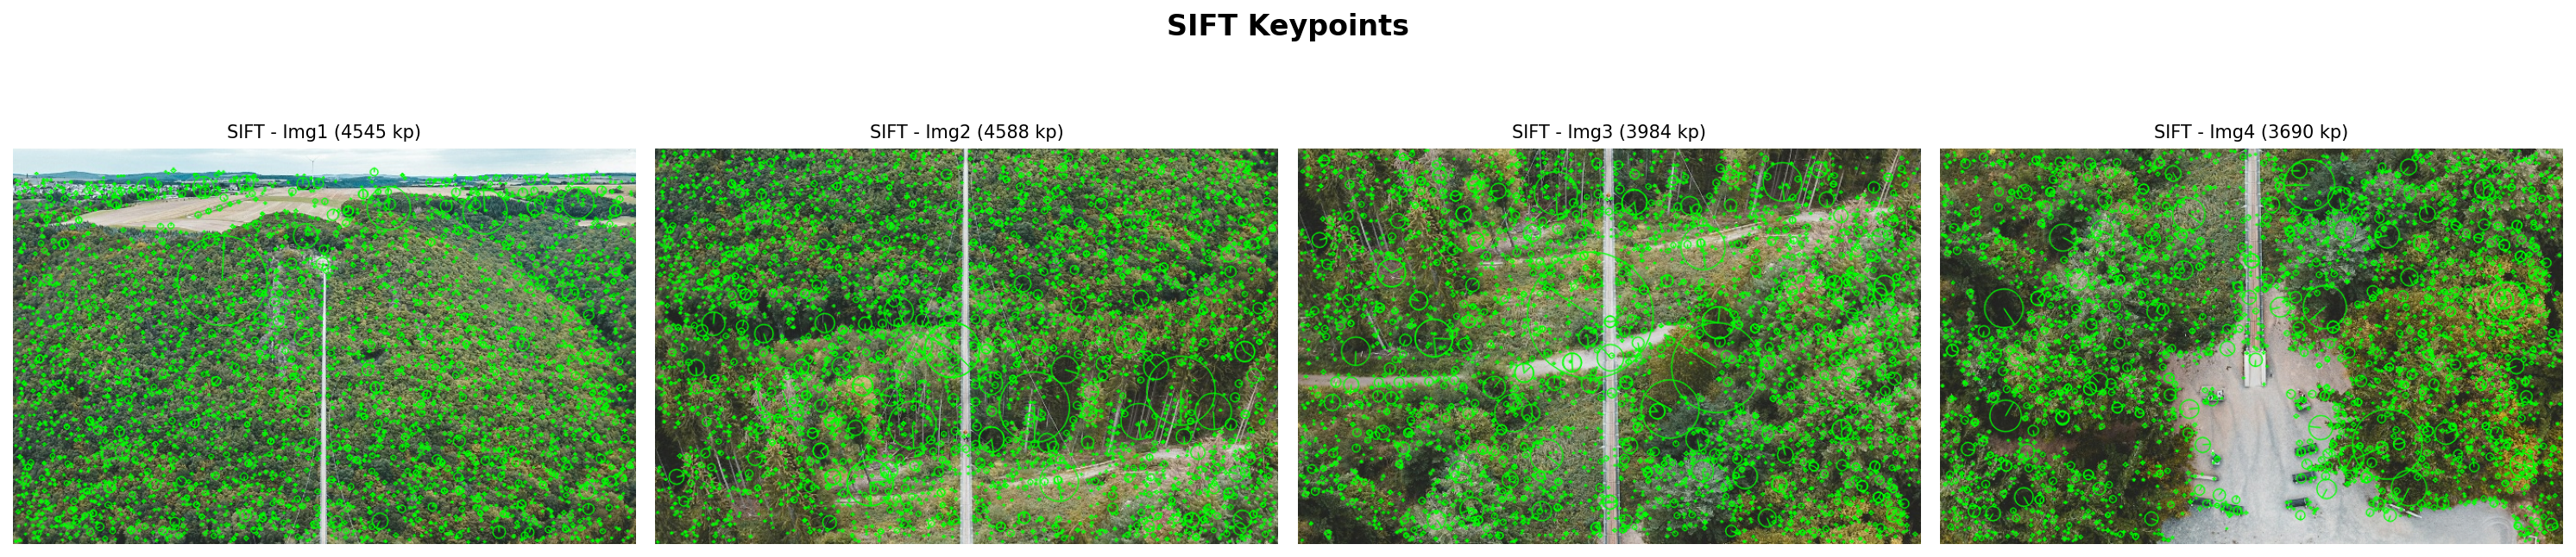
\includegraphics[width=0.9\textwidth]{results/part_c/keypoints_sift.png}
    \caption{SIFT keypoints extracted from the input images.}
    \label{fig:keypoints_sift}
\end{figure}

\begin{figure}[H]
    \centering
    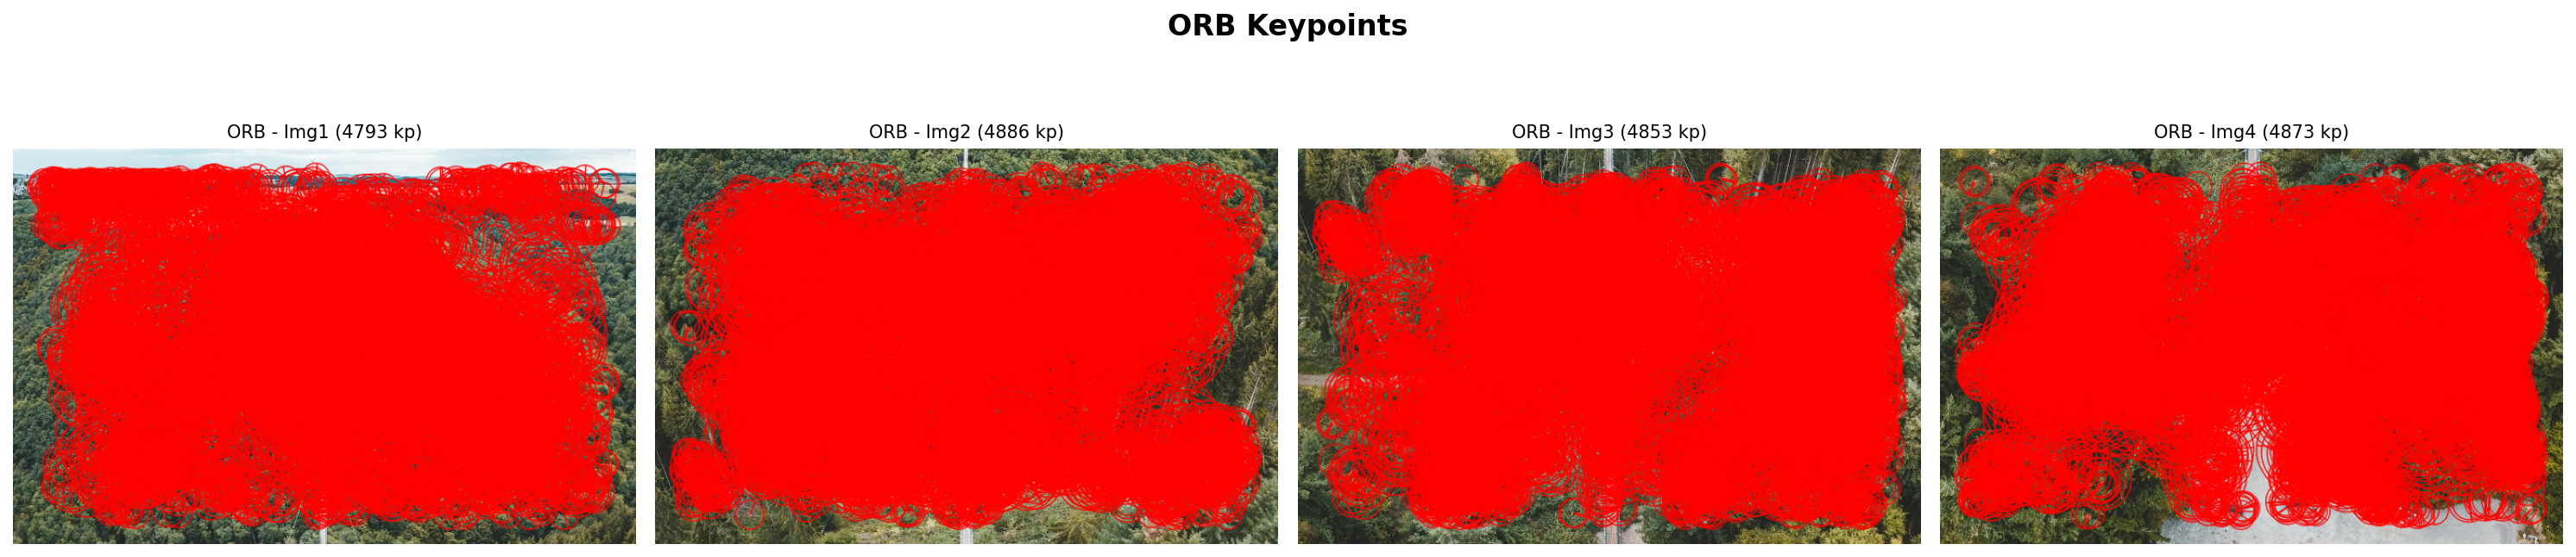
\includegraphics[width=0.9\textwidth]{results/part_c/keypoints_orb.png}
    \caption{ORB keypoints extracted from the input images.}
    \label{fig:keypoints_orb}
\end{figure}

% -------------------------------------------------------
\subsection{Feature Matching \& Lowe's Ratio Test}

Once descriptors are extracted, they must be paired. For SIFT, we compute the Euclidean distance ($L_2$ norm) between the 128-D vectors, often utilizing KD-Trees (like the FLANN matcher) for efficient high-dimensional nearest-neighbor searches. For ORB, we compute the Hamming distance (number of differing bits via hardware XOR) between the 256-bit strings, making ORB matching via a Brute-Force matcher (BFMatcher) computationally instantaneous.

\textbf{Lowe's Ratio Test:} Pure distance nearest-neighbor matching is heavily prone to false positives, especially in repetitive textures (like brick walls, windows, or clouds) where multiple descriptors might look identical. We apply Lowe's Ratio Test, proposed by David Lowe (inventor of SIFT)~\cite{lowe2004distinctive}:

\begin{equation}
    \frac{\text{Distance}(\text{Best\_Match})}{\text{Distance}(\text{Second\_Best\_Match})} < \tau
\end{equation}

A match is only accepted if the distance to the \textit{best} matching descriptor is significantly smaller (e.g., using threshold $\tau = 0.75$) than the distance to the \textit{second-best} descriptor. If the ratio is close to 1.0, it means the feature has another highly similar candidate nearby, indicating ambiguity. Filtering by this ratio mathematically guarantees the feature mapped is unique and unambiguous across the two images.

\textbf{Matched Features:}
Below are the mapped features between overlapping views using both SIFT and ORB matchers.

\begin{figure}[H]
    \centering
    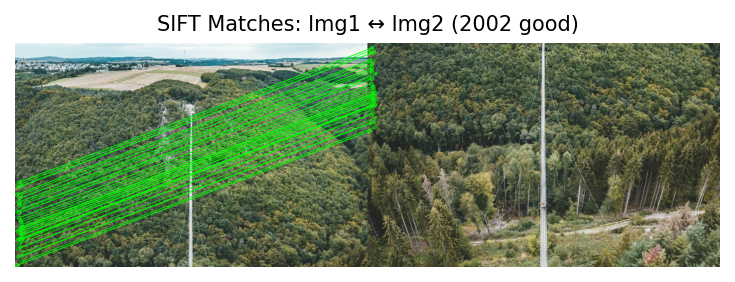
\includegraphics[width=0.95\textwidth]{results/part_c/matches_sift_12.png}
    \caption{SIFT feature matches between image pair 1--2.}
    \label{fig:matches_sift_12}
\end{figure}

\begin{figure}[H]
    \centering
    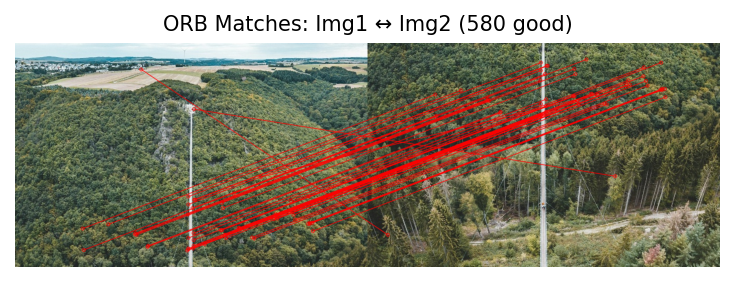
\includegraphics[width=0.95\textwidth]{results/part_c/matches_orb_12.png}
    \caption{ORB feature matches between image pair 1--2.}
    \label{fig:matches_orb_12}
\end{figure}

\begin{figure}[H]
    \centering
    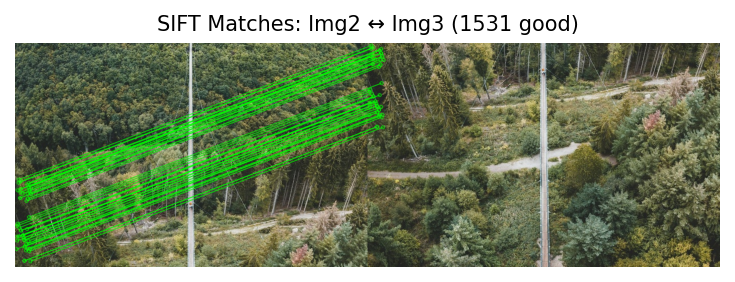
\includegraphics[width=0.95\textwidth]{results/part_c/matches_sift_23.png}
    \caption{SIFT feature matches between image pair 2--3.}
    \label{fig:matches_sift_23}
\end{figure}

\begin{figure}[H]
    \centering
    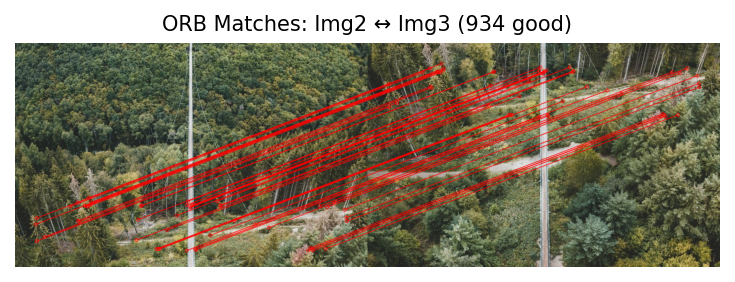
\includegraphics[width=0.95\textwidth]{results/part_c/matches_orb_23.png}
    \caption{ORB feature matches between image pair 2--3.}
    \label{fig:matches_orb_23}
\end{figure}

\begin{figure}[H]
    \centering
    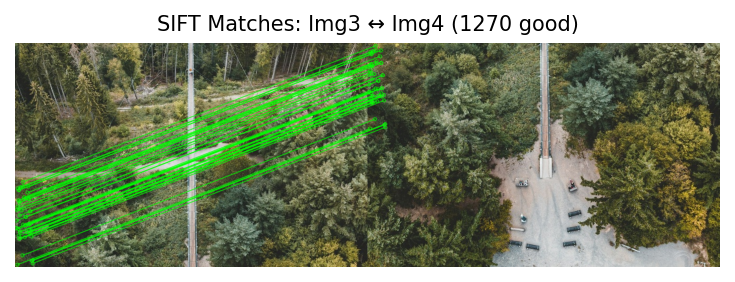
\includegraphics[width=0.95\textwidth]{results/part_c/matches_sift_34.png}
    \caption{SIFT feature matches between image pair 3--4.}
    \label{fig:matches_sift_34}
\end{figure}

\begin{figure}[H]
    \centering
    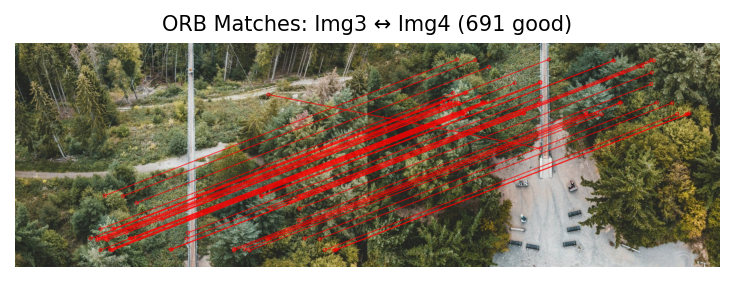
\includegraphics[width=0.95\textwidth]{results/part_c/matches_orb_34.png}
    \caption{ORB feature matches between image pair 3--4.}
    \label{fig:matches_orb_34}
\end{figure}

% -------------------------------------------------------
\subsection{Robust Homography Estimation (RANSAC)}

Even after distance and ratio filtering, incorrect geometric matches (outliers) will persist due to occlusions, moving objects, or similar patterns in different locations. To project View~2 into the coordinate frame of View~1, we must solve for the $3 \times 3$ Homography transformation matrix $\mathbf{H}$, which has 8 degrees of freedom:

\begin{equation}
    \begin{bmatrix} x' \\ y' \\ w' \end{bmatrix} = \begin{bmatrix} h_{11} & h_{12} & h_{13} \\ h_{21} & h_{22} & h_{23} \\ h_{31} & h_{32} & h_{33} \end{bmatrix} \begin{bmatrix} x \\ y \\ 1 \end{bmatrix} \quad \text{where} \quad X_{final} = \frac{x'}{w'}, Y_{final} = \frac{y'}{w'}
\end{equation}

A standard Least Squares solver would sum the error from all points, making it catastrophically skewed by even a single severe outlier. Instead, we rely on \textbf{RANSAC (Random Sample Consensus)}~\cite{fischler1981random}, which leverages a hypothesis-and-verify paradigm:

\begin{enumerate}
    \item \textbf{Hypothesize:} Randomly select a minimal subset of 4 matching point pairs (the minimum required to solve for $\mathbf{H}$).
    \item \textbf{Estimate:} Compute a candidate Homography matrix $\mathbf{H}_{candidate}$ using only these 4 points.
    \item \textbf{Verify:} Transform all other points from Image~2 using $\mathbf{H}_{candidate}$ and calculate their Euclidean distance to the corresponding points $(x_1, y_1)$ in Image~1 (Reprojection Error):
    \begin{equation}
        \text{Error} = \sqrt{(x_1 - X_{final})^2 + (y_1 - Y_{final})^2} < \epsilon
    \end{equation}
    \item \textbf{Consensus:} Count how many points have an error below a defined threshold $\epsilon$ (these are the \textit{inliers}).
\end{enumerate}

RANSAC iterates this process thousands of times. Ultimately, the mathematically optimal transformation is the single iteration that achieved maximum consensus (highest inlier count). The final $\mathbf{H}$ is then re-estimated using all inliers via Least Squares, completely neutralizing the disruptive influence of geometric outliers.

% -------------------------------------------------------
\subsection{Results \& Comparative Analysis}

The sequence of 4 input images was successfully unified structurally into a cohesive panorama using both pipelines.

\begin{figure}[H]
    \centering
    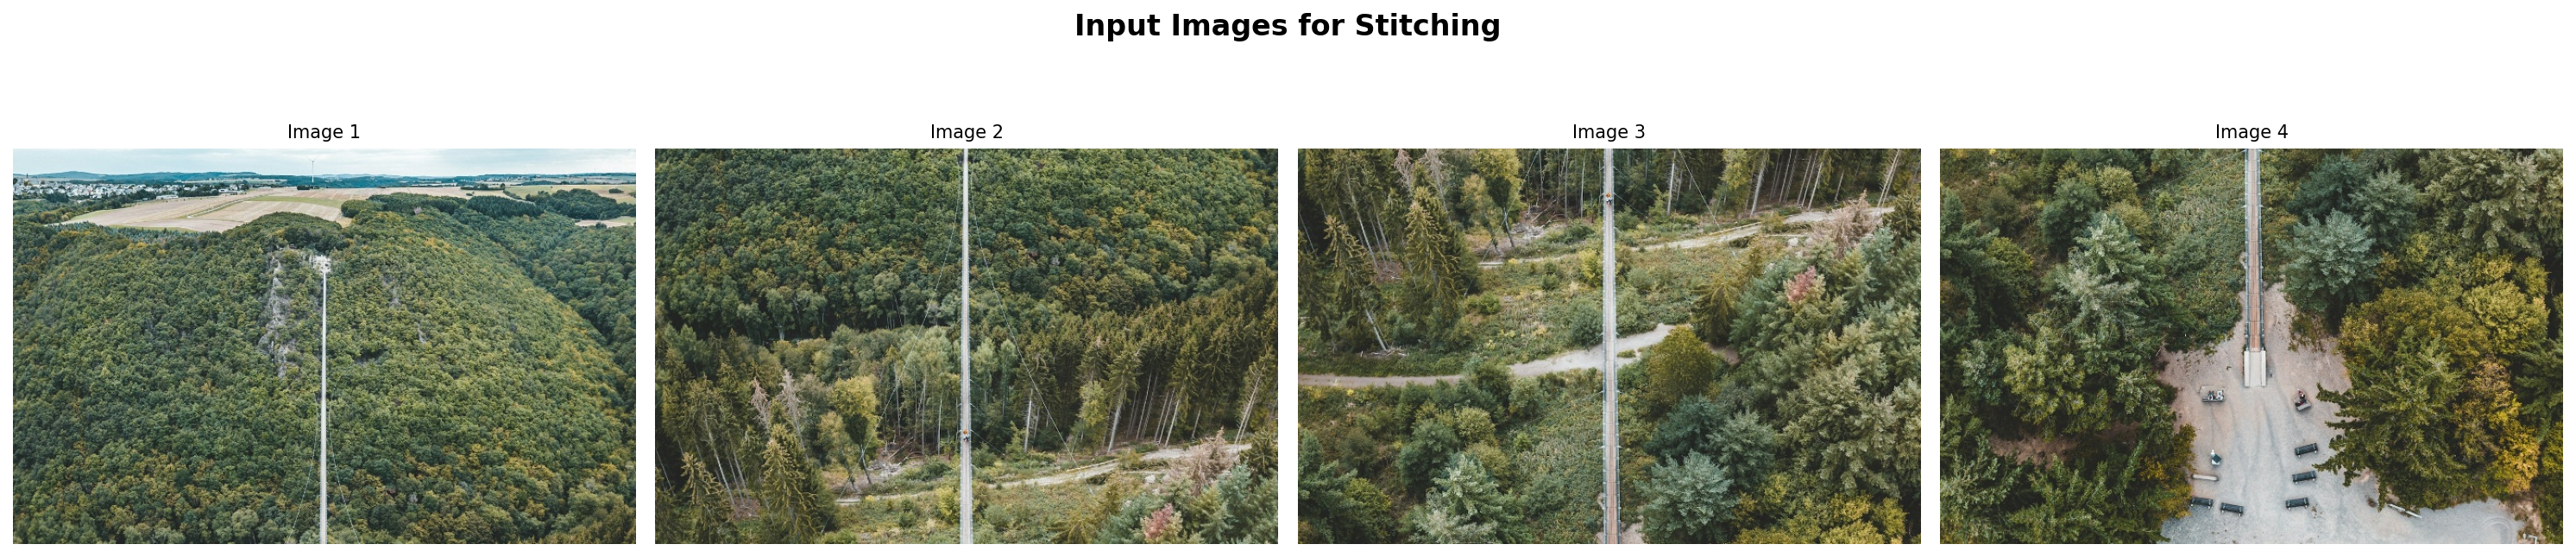
\includegraphics[width=0.95\textwidth]{results/part_c/input_images.png}
    \caption{The four input images used for panorama stitching.}
    \label{fig:input_images}
\end{figure}

\begin{figure}[H]
    \centering
    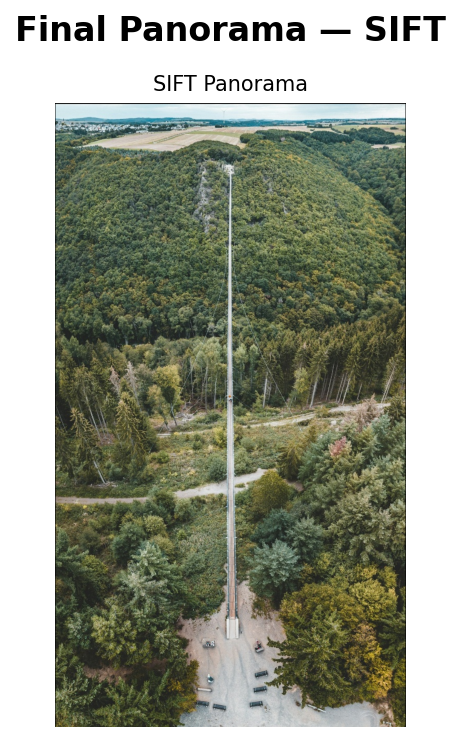
\includegraphics[width=0.95\textwidth]{results/part_c/panorama_sift_display.png}
    \caption{Final panorama generated using the SIFT pipeline.}
    \label{fig:panorama_sift}
\end{figure}

\begin{figure}[H]
    \centering
    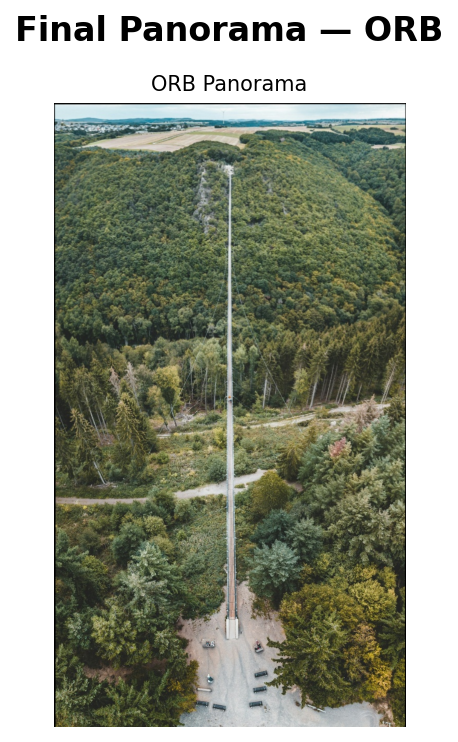
\includegraphics[width=0.95\textwidth]{results/part_c/panorama_orb_display.png}
    \caption{Final panorama generated using the ORB pipeline.}
    \label{fig:panorama_orb}
\end{figure}

\begin{figure}[H]
    \centering
    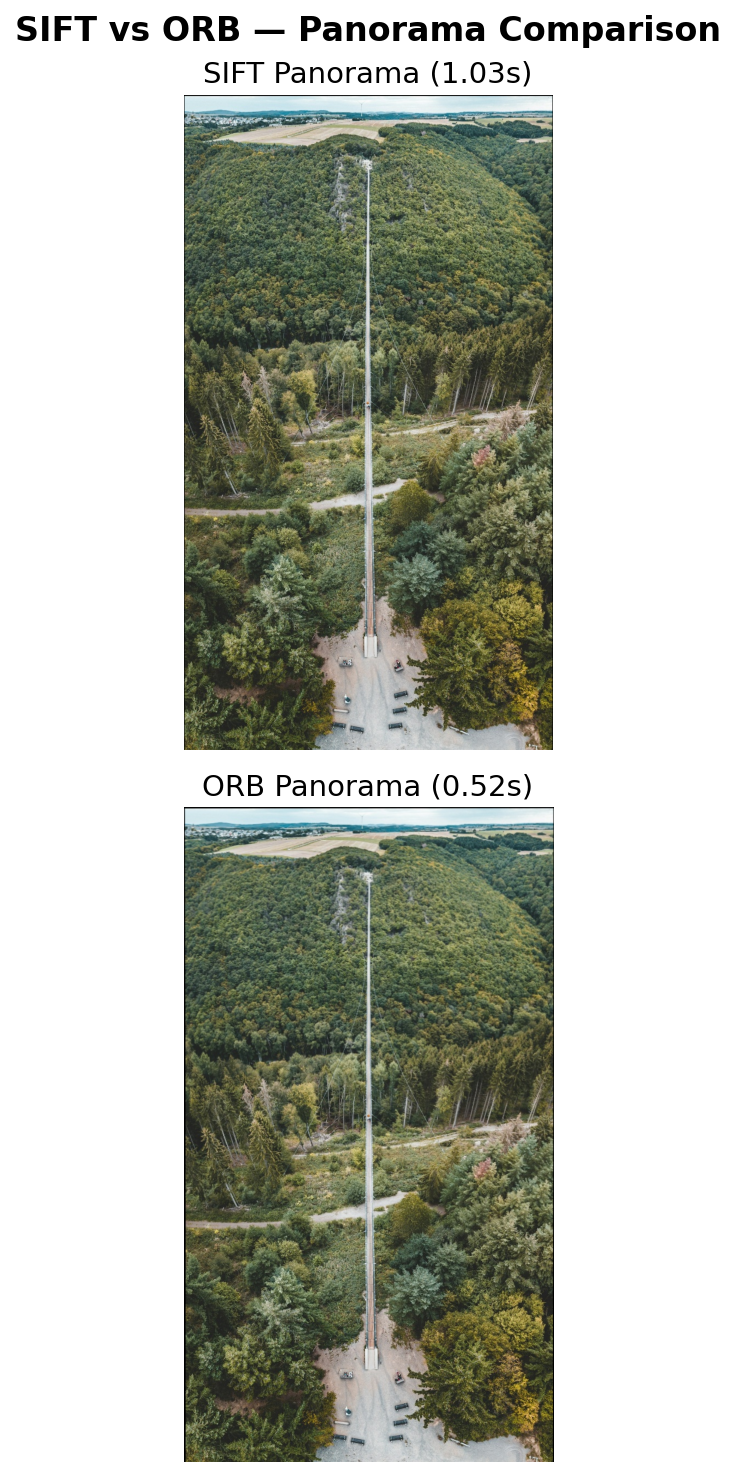
\includegraphics[width=0.95\textwidth]{results/part_c/panorama_comparison.png}
    \caption{Side-by-side comparison of SIFT and ORB panoramas.}
    \label{fig:panorama_comparison}
\end{figure}

We rigorously compared the two descriptors across 3 consecutive pairwise stitches.

\begin{figure}[H]
    \centering
    \includegraphics[width=0.85\textwidth]{results/analysis/part_c_matches_comparison.png}
    \caption{Match count comparison between SIFT and ORB across all image pairs.}
    \label{fig:matches_comparison}
\end{figure}

\begin{table}[H]
    \centering
    \caption{SIFT vs.\ ORB quantitative comparison across the full stitching pipeline.}
    \label{tab:sift_vs_orb}
    \begin{tabular}{lcc}
        \toprule
        \textbf{Metric} & \textbf{SIFT} & \textbf{ORB} \\
        \midrule
        Total Good Matches & \textbf{4,803} & \textbf{2,205} \\
        Total Inliers (RANSAC) & \textbf{4,790} & \textbf{2,162} \\
        Total Pipeline Time & \textbf{1.032s} & \textbf{0.520s} \\
        \bottomrule
    \end{tabular}
\end{table}

\begin{figure}[H]
    \centering
    \includegraphics[width=0.75\textwidth]{results/analysis/part_c_timing_comparison.png}
    \caption{Timing comparison: SIFT vs.\ ORB across all image pairs.}
    \label{fig:timing_comparison}
\end{figure}

\subsubsection{Match Density and Quality (SIFT's Advantage)}

SIFT dominated the extraction yield, computing \textbf{4,803} total good matches --- an impressive \textbf{2.18$\times$} more than ORB's \textbf{2,205} matches. SIFT's floating-point gradient histograms are heavily resilient to camera viewpoint shifting and scale changes, successfully pairing features even on the relatively structureless sky/cloud regions. Both descriptors maintained exceptionally high inlier ratios post-RANSAC (SIFT: 99.7\%, ORB: 98.1\%), confirming that Lowe's ratio test paired with RANSAC effectively enforces geometric purity regardless of the underlying descriptor mathematics.

\subsubsection{Computational Efficiency (ORB's Advantage)}

ORB completed the feature extraction and matching across all 3 overlapping pairs in \textbf{0.520s} versus SIFT's \textbf{1.032s} (a \textbf{2.0$\times$ speedup}). This acceleration is structural: computing simple binary intensity logic (ORB) on the CPU is vastly less computationally expensive than constructing Gaussian scale-space pyramids and integrating 128-dimensional floating-point vectors (SIFT).

\subsubsection{Practical Conclusion}

From an engineering perspective, RANSAC requires a strict minimum of only 4 valid corresponding points to compute a rigid Homography matrix. Therefore, ORB's ``lower'' yield of 2,205 matches is still overkill for high-quality geometric alignment. \textbf{ORB is unequivocally the superior architectural choice} for real-time video SLAM, autonomous drone mapping, and mobile applications where CPU/battery budgets are constrained.

However, standard ORB is notoriously susceptible to extreme scaling discrepancies. Therefore, \textbf{SIFT remains the mandatory standard} for high-precision, offline photogrammetry topologies (e.g., satellite imagery, medical tissue stitching) where scale-invariance and maximum descriptive robustness supersede processing time requirements.

% ============================================================
% 5. CONCLUSION AND POSSIBLE EXTENSIONS
% ============================================================
\section{Conclusion and Possible Extensions}

\subsection{Conclusion}

This midterm laboratory successfully conceptualized and implemented three independent computer vision pipelines spanning low-level processing to high-level geometric reconstruction. Through rigorous analytical and quantitative evaluation, we demonstrated that:

\begin{enumerate}
    \item \textbf{Spatial Filtering Optimality is Noise-Dependent}: The Median filter exhibits a structural advantage against impulse anomalies, achieving \textbf{33.36~dB} PSNR for Salt \& Pepper noise, but critically fails against systemic Gaussian degradation. Conversely, the Gaussian filter optimally suppresses systemic variance (up to \textbf{30.16~dB}) but requires bilateral edge-awareness to prevent boundary blurring.
    \item \textbf{Global Regularization Dominates Greedy Search in 3D Reconstruction}: Semi-Global Block Matching (SGBM) substantially improved structural fidelity over standard Block Matching across textureless regions via Markov Random Field energy minimization. With an acceptable 1.5$\times$ computational overhead, the pipeline achieved a dense recovery of \textbf{103,441} globally coherent 3D points.
    \item \textbf{Feature Matching Requires Application-Specific Trade-offs}: In multi-view panorama generation, SIFT provides exhaustive scale-invariant accuracy (yielding 2.18$\times$ more matches), making it ideal for offline photogrammetry. Conversely, ORB's binary intensity logic executes 2.0$\times$ faster while still surpassing necessary RANSAC thresholds, rendering it superior for real-time mobile SLAM applications.
\end{enumerate}

\subsection{Possible Extensions \& Future Work}

While the implemented algorithms establish robust baselines, these foundational methods expose vectors for advanced optimization and contemporary deep-learning enhancements:

\subsubsection{Part A Extensions: Advanced Restoration}
\begin{itemize}
    \item \textbf{Adaptive Filtering:} Upgrading from statically-sized kernels to spatially additive filters (e.g., Adaptive Wiener Filters) that automatically compute local signal variance $\sigma^2$ before blurring, thereby providing mathematically optimal noise suppression per pixel.
    \item \textbf{Deep Denoising Autoencoders:} Replacing classical convolution matrices with a convolutional neural network (CNN). Training an encoder-decoder architecture (e.g., U-Net) on pairs of synthetic noisy and clean images to recognize and procedurally remove non-Gaussian, non-uniform noise arrays.
\end{itemize}

\subsubsection{Part B Extensions: Deep Depth Perception}
\begin{itemize}
    \item \textbf{WLS Disparity Filtering:} Applying a Weighted Least Squares (WLS) post-processing filter based on the left-view's guided image gradient. This mathematical refinement forces the depth map edges to perfectly align with the color image borders.
    \item \textbf{End-to-End Neural Stereo:} Implementing a modern deep stereo network (e.g., RAFT-Stereo or PSMNet) that constructs a 4D correlation volume and iteratively converges on dense sub-pixel disparities, effectively neutralizing the ``textureless regions'' problem by learning high-level contextual semantics.
\end{itemize}

\subsubsection{Part C Extensions: Seamless Immersion}
\begin{itemize}
    \item \textbf{Multi-Band Laplacian Blending:} Currently, naive alpha-blending across homography seams produces hard ``ghosting'' artifacts and exposure inconsistencies. Leveraging Laplacian pyramid blending separates the image into high and low spatial frequencies---seamlessly blending broad exposure gradients on low levels while retaining razor-sharp stitched edges on high levels.
    \item \textbf{Bundle Adjustment \& Spherical Warping:} Standard homography transformation projects all frames linearly onto an infinite 2D plane, causing severe stretching distortions mathematically inherent at the panorama's extremities. Projecting coordinates onto a cylinder or sphere, followed by a non-linear Least Squares `Bundle Adjustment' of all camera parameters simultaneously, would permit infinite $360^{\circ}$ topological panoramas.
\end{itemize}

% ============================================================
% REFERENCES
% ============================================================
\begin{thebibliography}{9}

\bibitem{hirschmuller2005accurate}
Hirschm\"uller, H. (2005).
``Accurate and Efficient Stereo Processing by Semi-Global Matching and Mutual Information.''
\textit{IEEE Conference on Computer Vision and Pattern Recognition (CVPR)}, pp.~807--814.

\bibitem{lowe2004distinctive}
Lowe, D.\,G. (2004).
``Distinctive Image Features from Scale-Invariant Keypoints.''
\textit{International Journal of Computer Vision}, 60(2), pp.~91--110.

\bibitem{rublee2011orb}
Rublee, E., Rabaud, V., Konolige, K., \& Bradski, G. (2011).
``ORB: An Efficient Alternative to SIFT or SURF.''
\textit{IEEE International Conference on Computer Vision (ICCV)}, pp.~2564--2571.

\bibitem{fischler1981random}
Fischler, M.\,A. \& Bolles, R.\,C. (1981).
``Random Sample Consensus: A Paradigm for Model Fitting with Applications to Image Analysis and Automated Cartography.''
\textit{Communications of the ACM}, 24(6), pp.~381--395.

\bibitem{wang2004image}
Wang, Z., Bovik, A.\,C., Sheikh, H.\,R., \& Simoncelli, E.\,P. (2004).
``Image Quality Assessment: From Error Visibility to Structural Similarity.''
\textit{IEEE Transactions on Image Processing}, 13(4), pp.~600--612.

\bibitem{bradski2000opencv}
Bradski, G. (2000).
``The OpenCV Library.''
\textit{Dr.\ Dobb's Journal of Software Tools}.

\bibitem{tomasi1998bilateral}
Tomasi, C., \& Manduchi, R. (1998).
``Bilateral Filtering for Gray and Color Images.''
\textit{Sixth International Conference on Computer Vision (ICCV)}, pp.~839--846.

\bibitem{longuet1981computer}
Longuet-Higgins, H.\,C. (1981).
``A Computer Algorithm for Reconstructing a Scene from Two Projections.''
\textit{Nature}, 293(5828), pp.~133--135.

\end{thebibliography}

\end{document}